%
% The point of the chapter introduction is to set the scence and explain what you are doing and why.
% Problems that i am tackling here are: Explaining someone might get different results while using the same method with the same configuration this is for the deep learning method.
% If you are going to do a comparison with another method on a different dataset what parameters should you consider changing and apadting and which are less important.
% This is the first time that such a large scale evaluation has been performed in Target Dependent Sentiment analysis and is the first to do it over different domain, type and medium.
%
% The normal question of why did we choose these three different methods:
% 1. Is a deep learning that has been cited many times and reprduced and repeated with different result thus it would be interesting to be able to give a reason why the results are different.
% 2. The linear model allow comparison of more traditional features like the importance of sentiment lexicons and dependency parsers. As we are comparing to models that are the same apart from a dependency parser weather the difference is statitsically signifcant as this was never shown in the original paper.
%
%
%%%%% Need to explain somewhere the reason why it is still important to replicate a method when the code has already been released. I put this as the following within the presentation as COLING: Reproducing methods that have released their code is still a worth while pursuit as reproducing the method from the paper allows us as a community to find out what is missing in our papers that is vital for reproducing our work.

The evaluation of different methods has become more problematic over the years as more ever increasingly complex methods have come about. Therefore the importance of comparative evaluation becomes ever more important. Comparative evaluation can become more challenging when the evaluation is across multiple datasets with different properties for example different domain (politics, electronics), medium (spoken text, written), and type (social media, review). Each one these properties may cause adjustments in the methods to get a fair comparison, for example a method that uses a dependency parser may perform significantly better when the parser being used has been created for the data that it is being applied too rather than a different data type/domain/medium. Therefore knowing what changes to a method that are significant to its performance given the dataset properties is important for fair comparison. This is crucial with respect to comparing previous state of the art results that have a different evaluation setup e.g. use a different word embedding, dependency parser, tokeniser etc. Thus one major contribution of this section is quantifying the importance of evaluation setup, by evaluating methods across numerous different parameters/settings of the methods across different datasets that contain different properties. This is of great importance as some methods have used domain specific settings e.g. word embeddings \citep{vo2015target,zhang2016gated,wang-etal-2017-tdparse} and are therefore not comparable to methods that do not \citep{chen-etal-2017-recurrent,li-etal-2018-transformation} unless they are re-run or reproduced. Therefore quantifying the difference in methods between these domain specific settings could allow comparability without the need for re-running or reproducing.
Furthermore knowing which parameters/settings affects the methods can help guide future researchers and practitioners choose sensible default parameters/settings before adapting the methods to their own needs.
\todo[inline]{A potential research questions is What properties within a method are significantly important to the performance of the method and how they relate to different dataset properties?}
\\
% This paper: Target-Sensitive Memory Networks for Aspect Sentiment Classification
% Must have reproduced the work from Wang et al 2016 which is the ATAE method as they show macro F1 scores but the original only looked at accuracy.
Another equally important and related problem is that of reproducability. Some work within Target Dependent Sentiment Analysis (TDSA) reproduce or re-use the code of previous works to circumnavigate\comment{is avoid a better word?} the evaluation setup problem stated above \citep{chen-etal-2017-recurrent,tay2018learning}. However this can be shown to be difficult through a couple of works \citep{chen-etal-2017-recurrent,tay2018learning} that could not re-run or replicate respectively successfully one particular deep learning method \citet{tang-etal-2016-effective} when using the same datasets and evaluation setup. In this chapter we show a potential reason why this maybe the case, as well as highlighting other important parameters/settings that are missing from the original papers that are critical to replicating the three chosen methods. This chapter also shows the (obvious?) relation between significantly important parameters/settings and the parameters that are stated within the paper to allow others to successfully replicate the method.\\
\\
% Need to add into this paragraph something to do with generalisability I think with regards to the evaluation across numerous datasets and the results from that.
The chapter concludes with a mass evaluation across multiple datasets on the methods that have been replicated within the chapter using the optimal parameters found for each method on each dataset. This mass evaluation will be a first within TDSA as the English datasets will come from three different dataset properties; 1. domain, 2. type, and 3. medium. From this the community can have a strong baseline of methods to compare to across all of these datasets. This will also be the first time the community will know the true general State Of The Art (SOTA) within TDSA as previous results only state their results for a limited number of datasets and therefore are not general enough to compare to.\\
\\
In summary this chapter demonstrates the importance of parameters within TDSA methods and how these relate to the replicability of the method from the paper. Lastly it highlights the under utilisation of English datasets within TDSA and the importance of them with regards to generalisability of methods within TDSA. The chapter is structured as follows; first explain the three different methods that are being replicated. The second section shows how they were successfully replicated. The third section reveals the importance of different parameters within a method and the importance of these parameters in replicating the original work. The last section presents the mass evaluation results.

\section{Methods}
\label{section:repro_methods}
% In this section I need to introduce the three methods that I am going to replicate, the reason these were chosen other than they are popular within the literature. Then go throught each method explaining the method and showing a diagram of the method.

In this chapter we replicate three popular methods; \cite{vo2015target}, \cite{wang-etal-2017-tdparse}, and \cite{tang-etal-2016-effective}. This section will describe each model in detail in the order just given and will conclude with the reason of why these three were chosen.

%
% Got to this point in writing
%

%of which the first two use linear Support Vector Machines (SVM) while the last is a non-linear Long Short Term Memory (LSTM) Neural Network (NN) model. These three methods were chosen due to the difference in approach; NN compared to SVM, the use of 

%We first explain each method we replicated, and show how we have successfully replicated the methods on the datasets they were originally evaluated on. We then 

%We then expand the evaluation setup to include more datasets to increase the coverage and generalisability of the results from these methods. Using this expanded evaluation setup we explore the importance of different parts of these methods and outline which are the most volatile to change with respect to the results. Furthermore due to the increase in the expanded datasets we can find out whether different parameter are more sensitive to different domains, mediums, and/or types.  

\subsection{\cite{vo2015target}}
%  They take the word vectors of the left and right side of the target word, as well as the target word and full text.
This is simplest of the three methods being presented within the chapter. As shown in figure \ref{fig:repro_vo_method} it treats each word in the sentence as a word vector that has come from a pre-trained word vector model e.g. Glove \citep{pennington-etal-2014-glove}. From this the method splits the sentence into four different contexts based on the target word(s) position:
\begin{enumerate}
    \item The whole context -- The whole sentence.
    \item The left context -- all words left of the target word but not including the target word.
    \item The target context -- the target word(s) (can be more than word e.g. camera lens).
    \item The right context -- all words right of the target word but not including the target word.
\end{enumerate}
From these variable length contexts, numerous Neural Pooling (NP) methods are applied to these contexts, to create fixed length feature vectors from a variable length sentence. A NP method as stated takes a variable number of word vectors e.g. $W \in  \mathbb{R}^{d\times n}$ where $n$ is the number of words and $d$ is the dimension of the word vector which represent features of the word. The NP then applies a pooling method e.g. maximum value across all the $d$ dimensions of the $n$ words to output a feature vector of $w \in \mathbb{R}^{d}$ in the example. For each context and NP method a feature vector is created, all feature vectors are then concatenated and are inputted into the linear Support Vector Machine (SVM) to classify the sentiment of the target.\\
\\

The method described above is the general approach \citet{vo2015target} took. More specifically they created four different methods which all used the same NP method but different contexts and one also incorporated sentiment lexicons in a novel way, these are described below:
\begin{enumerate}
    \item Target-Independent -- Only used the whole context.
    \item Target-Dependent Minus - Left, right, and target contexts.
    \item Target-Dependent - Left, right, target, and whole contexts (Union of the first two methods).
    \item Target-Dependent Plus - This incorporated sentiment lexicons by filtering all words that are not in the sentiment lexicon from a given context. This sentiment filtering was applied to the left and right contexts denoted as \textit{LS} and \textit{RS} respectively. In total this method used the left, right, target, whole, \textit{LS}, and \textit{RS} contexts.
\end{enumerate}
As can be seen above each method from the top of the list incorporates more context or external information as you move down the list of methods. Furthermore from the methods above only the first method will always produce the same sentiment no matter the target word if all targets come from the same sentence, as it does not incorporate any target information.\\
There are several contribution of this paper; first is the splitting up of the sentence into different contexts to model simple interaction between the different contexts. Second the use of sentiment lexicons to filter words when the words are represented as word vectors within sentiment analysis. Lastly the extension of NP methods from \citet{tang-etal-2014-learning} original \textit{max}, \textit{min}, and \textit{avg} functions to the those listed below with the contribution of also explaining what the functions capture with regards to sentiment:
\begin{enumerate}
    \item \textit{max} - Maximum value represents positive sentiment.
    \item \textit{min} - Minimum value represents negative sentiment.
    \item \textit{avg} - Average value represents the average sentiment.
    \item \textit{std} - Standard deviation represents the sentiment variation.
    \item \textit{pro} - Product represents the average sentiment but with larger differences between positive and negative sentiment.
\end{enumerate}

%This is the first and most simple of the Neural Pooling (NP) methods that has been applied to TDSA. They create different contexts from the text and for each of these contexts they perform maximum, minimum, average, standard deviation, and product pooling over the word embeddings. These pooling features are then inputted into a Support Vector Machine (SVM) to classify the text.

%They created four main contexts that made up four different methods they tested to show the importance of these different contexts. The four main methods and their contexts are explained below:
%\begin{enumerate}
%    \item \textbf{Target-Ind} -- Only the full text contexts.
%    \item \textbf{Target-Dep}- -- Left and right context of the target word and the target word context.
%    \item \textbf{Target-Dep} -- The full text contexts as well as the contexts of \textbf{Target-Dep-}
%    \item \textbf{Target-Dep+} -- All the contexts of \textbf{Target-Dep} as well as additional left and right context where the embeddings are only of the words that appear in the given sentiment lexicon (LS and RS contexts).
%\end{enumerate}
%As might be obvious each method tends to improve upon the other be including more contexts. Furthermore the \textbf{Target-Ind} method is the only method above that will not produce a different sentiment score if two targets are in the same sentence, as it only contains sentence level features and no target specific features. These different contexts are also explained through figure \ref{fig:repro_vo_method}.
\begin{figure}[!ht]
    \begin{tikzpicture}[
    feature/.style={circle, draw, radius=0.05},
    vector/.style={rectangle, draw, minimum height=1cm},
    arrow_pointer/.style={decoration={markings,mark=at position 1 with %
    {\arrow[scale=3,>=stealth]{>}}},postaction={decorate}}]
    
    % Left Context
    \node[feature](feat1){};
    \node[feature, below=.2 of feat1](feat2){};
    \node[feature, above=.2 of feat1](feat0){};
	\node[vector, fit=(feat0)(feat1)(feat2)] (vec0) {};
	\node[below=.1 of vec0] (x0) {$w_0$};
	
	\node[feature, right=.5 of vec0](feat4){};
    \node[feature, below=.2 of feat4](feat5){};
    \node[feature, above=.2 of feat4](feat3){};
	\node[vector, fit=(feat4)(feat3)(feat5)] (vec1) {};
	\node[below=.1 of vec1] (x1) {$w_1$};
	
	\node[right=.5 of vec1](dot0){$\dots$};
	
	\node[feature, right=.5of dot0](feat7){};
    \node[feature, below=.2 of feat7](feat8){};
    \node[feature, above=.2 of feat7](feat6){};
	\node[vector, fit=(feat7)(feat6)(feat8)] (vec2) {};
	\node[below=.1 of vec2] (x2) {$w_l$};
	
	\node[below left=.1 of x0] (line0) {};
	\node[below right=.1 of x2] (line1) {};
	\draw [|-|] (line0) -- (line1)  node[pos=0.5, below=0.1]{Left Context};
	
	% Target Context
	\node[feature, right=.8 of vec2](feat10){};
    \node[feature, below=.2 of feat10](feat11){};
    \node[feature, above=.2 of feat10](feat9){};
	\node[vector, fit=(feat10)(feat9)(feat11)] (vec3) {};
	\node[below=.1 of vec3] (x3) {$w_{l+1}$};
	
	\node[right=.5 of vec3](dot1){$\dots$};
	
	\node[feature, right=.5 of dot1](feat13){};
    \node[feature, below=.2 of feat13](feat14){};
    \node[feature, above=.2 of feat13](feat12){};
	\node[vector, fit=(feat13)(feat12)(feat14)] (vec4) {};
	\node[below=.1 of vec4] (x4) {$w_{r-1}$};
	
	\node[below left=.1 of x3] (line2) {};
	\node[below right=.1 of x4] (line3) {};
	\draw [|-|] (line2) -- (line3)  node[pos=0.5, below=0.1]{Target Context};
	
	% Right Context
	\node[feature, right=.8 of vec4](feat16){};
    \node[feature, below=.2 of feat16](feat17){};
    \node[feature, above=.2 of feat16](feat15){};
	\node[vector, fit=(feat16)(feat15)(feat17)] (vec5) {};
	\node[below=.1 of vec5] (x5) {$w_r$};
	
	\node[right=.5 of vec5](dot2){$\dots$};
	
	\node[feature, right=.5 of dot2](feat19){};
    \node[feature, below=.2 of feat19](feat20){};
    \node[feature, above=.2 of feat19](feat18){};
	\node[vector, fit=(feat19)(feat18)(feat20)] (vec6) {};
	\node[below=.1 of vec6] (x6) {$w_{n-1}$};
	
	\node[feature, right=.5 of vec6](feat22){};
    \node[feature, below=.2 of feat22](feat23){};
    \node[feature, above=.2 of feat22](feat21){};
	\node[vector, fit=(feat22)(feat21)(feat23)] (vec7) {};
	\node[below=.1 of vec7] (x7) {$w_n$};
	
	\node[below left=.1 of x5] (line4) {};
	\node[below right=.1 of x7] (line5) {};
	\draw [|-|] (line4) -- (line5)  node[pos=0.5, below=0.1]{Right Context};
	
	\node[below=.5 of line0] (line6) {};
	\node[below=.5 of line5] (line7) {};
	\draw [|-|] (line6) -- (line7)  node[pos=0.5, below=0.1]{\textbf{Full Context}};
	
	\node[rectangle, draw, minimum width=3em, above=1.9, fit={(vec0.west) (vec7.east)}, minimum height = 1cm, inner ysep=0pt, label={center:Pooling (Max, Min, Prod, Std, Avg)}] (pooling) {};
	
	% Arrows for the context to the pooling layer
	% Left context
	\node[above=.3 of dot0] (top_dot0) {};
	\node[above=1.2 of dot0] (top_top_dot0) {};
	\draw [arrow_pointer] (top_dot0) -- (top_top_dot0);
	
	% Center context
	\node[above=.3 of dot1] (top_dot1) {};
	\node[above=1.2 of dot1] (top_top_dot1) {};
	\draw [arrow_pointer] (top_dot1) -- (top_top_dot1);
	
	% Right context
	\node[above=.3 of dot2] (top_dot2) {};
	\node[above=1.2 of dot2] (top_top_dot2) {};
	\draw [arrow_pointer] (top_dot2) -- (top_top_dot2);
	
	\node[rectangle, draw, minimum width=3em, above=3.8, fit={(vec0.west) (vec7.east)}, minimum height = 1cm, inner ysep=0pt, label={center:SVM}] (svm) {};
	\draw [arrow_pointer] (pooling) -- (svm);
\end{tikzpicture}


    \caption{General architecture of \citet{vo2015target}}
    \label{fig:repro_vo_method}
\end{figure}
\newpage


%  sentence into different contexts to model simple interaction between the different contexts.
\subsection{\cite{wang-etal-2017-tdparse}}
Is a direct extension of \cite{vo2015target} where they keep the same NP methods and general architecture but change the contexts. The main motivation of \citet{wang-etal-2017-tdparse} method is to improve the simple interaction of the different contexts by incorporating the syntactic structure of the target word using a dependency parser. In more detail this dependency context contains the target word and all connected words within the same root. This makes the assumption that the dependency parser that is used can create multiple roots from one text as it assumes the text is made of more than one sentence. If the dependency parser does not create more than one root in a text then the dependency context will be the same as the whole context from \citet{vo2015target} method. The dependency parser they therefore used was the TweeboParser \citep{kong-etal-2014-dependency} which was created for noisy text like Tweets and hence why multiple roots can occur in one text. This parser was also used because it was especially created for noisy text and the datasets \citet{wang-etal-2017-tdparse} applied this method to were Twitter datasets.

As with \citet{vo2015target}, \citet{wang-etal-2017-tdparse} had three different models each containing either more contexts or external information, these are describe in more detail below:
\begin{enumerate}
    \item TDParse Minus -- Only used the dependency context.
    \item TDParse -- Left, right, target, and dependency contexts.
    \item TDParse Plus -- Left, right, target, dependency, \textit{LS}, and \textit{RS} contexts.
\end{enumerate}

\subsection{\cite{tang-etal-2016-effective}}
%[I may need the reference to the LSTM cell???]
Unlike the previous two methods this is a Neural Network (NN) method, of which it was the first for TDSA to use a Long Short Term Memory (LSTM) NN \citep{hochreiter1997long}. Similar to the other two methods \citet{tang-etal-2016-effective} created three different methods; 1. Standard LSTM (LSTM), 2. Target Dependent LSTM (TDLSTM), and 3. Target Connected LSTM (TCLSTM).\\

The LSTM method is the most basic approach and can be seen in full in figure \ref{fig:repro_lstm_method}. It treats each word within the text as a word vector where the word vector can be either randomly initialised or initialised from a pre-trained word vector model. The word representations are then inputted into the LSTM NN which takes the word representation from the left most word first to the last word in the sentence. The output from the LSTM at the last word in the sentence ($h_n$) is fed into a linear layer with a softmax activation function to generate the probability of the sentiment of the text. This method can be seen in figure. This method takes no target context into account, therefore it represents a sentence level sentiment classifier, and was used as the baseline method in \citet{tang-etal-2016-effective}\\
\begin{figure}[!ht]
    \centering
    \begin{tikzpicture}[
    feature/.style={circle, draw, radius=0.05},
    vector/.style={rectangle, draw, minimum height=1cm},
    lstm_node/.style={rectangle, draw},
    arrow_pointer/.style={decoration={markings,mark=at position 1 with %
    {\arrow[scale=1,>=stealth]{>}}},postaction={decorate}}]
    
    % Whole Context
    \node[feature](feat1){};
    \node[feature, below=.2 of feat1](feat2){};
    \node[feature, above=.2 of feat1](feat0){};
	\node[vector, fit=(feat0)(feat1)(feat2)] (vec0) {};
	\node[below=.1 of vec0] (x0) {$w_0$};
	% LSTM 0
	\node[lstm_node, above=1.5 of feat1](lstm0){LSTM};
	\draw [arrow_pointer] (vec0) -- (lstm0);
	
	\node[right=1 of feat1](dot0){$\dots$};
	
	\node[feature, right=1 of dot0](feat4){};
    \node[feature, below=.2 of feat4](feat5){};
    \node[feature, above=.2 of feat4](feat3){};
	\node[vector, fit=(feat4)(feat3)(feat5)] (vecn) {};
	\node[below=.1 of vecn] (xn) {$w_n$};
	% LSTM n
	\node[lstm_node, above=1.5 of feat4](lstmn){LSTM};
	\draw [arrow_pointer] (vecn) -- (lstmn);
	
	% Arrows between LSTMs
	\node[right=.5 of lstm0] (lstm0_left_mid) {};
	\node[left=.5 of lstmn] (lstm0_right_mid) {};
	\draw [arrow_pointer] (lstm0) -- (lstm0_left_mid) node[pos=0.5, below=0.1]{$h_1$};
	\draw[dotted](lstm0_left_mid) -- (lstm0_right_mid);
	\draw [arrow_pointer] (lstm0_right_mid) -- (lstmn) node[pos=0.5, below=0.1]{$h_{n-1}$};
	
	% Softmax
	\node[rectangle, draw, above = of lstmn] (softmax) {Softmax};
	\draw [arrow_pointer] (lstmn) -- (softmax) node[pos=0.5, left=0.05]{$h_{n}$};
	
	
	% Whole context arrows
	\node[below left=.1 of x0] (line0) {};
	\node[below right=.1 of xn] (linen) {};
	\draw [|-|] (line0) -- (linen)  node[pos=0.5, below=0.1]{Whole Context};

\end{tikzpicture}
    \caption{Architecture of the LSTM method.}
    \label{fig:repro_lstm_method}
\end{figure}

The TDLSTM which can be seen in figure \ref{fig:repro_tdlstm_method} is a target specific model, it splits the sentence into two contexts:
\begin{enumerate}
    \item Left context -- The words left of the target word, including the target itself.
    \item Right context -- The words right of the target word, including the target itself.
\end{enumerate}
Each context has it's own LSTM, the left has an LSTM that takes words representation from left to right, and the right LSTM takes words representation from right to left. The last word representation(s) that are input into both LSTMs are the target word's, this was so that the LSTM could better model the sentiment of the sentence with regard to the target word(s). The final output of both LSTMs ($h_{r-1}$, $h_{l+1}$) are concatenated together, which is fed into a linear layer with a softmax activation function to generate the probability of the sentiment of the text.\todo{The TDLSTM diagram might be better on a whole horizontal page?}

\begin{figure}[!ht]
    \centering
    \resizebox{11.0cm}{!}{%
\begin{tikzpicture}[
    feature/.style={circle, draw, radius=0.05},
    vector/.style={rectangle, draw, minimum height=1cm},
    lstm_node/.style={rectangle, draw},
    arrow_pointer/.style={decoration={markings,mark=at position 1 with %
    {\arrow[scale=1,>=stealth]{>}}},postaction={decorate}}]
    
    % Left Context
    \node[feature](feat1){};
    \node[feature, below=.2 of feat1](feat2){};
    \node[feature, above=.2 of feat1](feat0){};
	\node[vector, fit=(feat0)(feat1)(feat2)] (vec0) {};
	\node[below=.1 of vec0] (x0) {$w_0$};
	% LSTM 0
	\node[lstm_node, above=1.5 of feat1](lstm0){LSTM};
	\draw [arrow_pointer] (vec0) -- (lstm0);
	
	\node[right=1 of feat1](dot0){$\dots$};
	
	\node[feature, right=1 of dot0](feat4){};
    \node[feature, below=.2 of feat4](feat5){};
    \node[feature, above=.2 of feat4](feat3){};
	\node[vector, fit=(feat4)(feat3)(feat5)] (vec1) {};
	\node[below=.1 of vec1] (x1) {$w_l$};
	% LSTM 1
	\node[lstm_node, above=1.5 of feat4](lstm1){LSTM};
	\draw [arrow_pointer] (vec1) -- (lstm1);
	
	% Arrows between LSTMs
	\node[right=.5 of lstm0] (lstm0_left_mid) {};
	\node[left=.5 of lstm1] (lstm0_right_mid) {};
	\draw [arrow_pointer] (lstm0) -- (lstm0_left_mid) node[pos=0.5, below=0.1]{$h_1$};
	\draw[dotted](lstm0_left_mid) -- (lstm0_right_mid);
	\draw [arrow_pointer] (lstm0_right_mid) -- (lstm1) node[pos=0.5, below=0.1]{$h_{l-1}$};
	
	
	
	\node[feature, right=1.2 of feat4](feat7){};
    \node[feature, below=.2 of feat7](feat8){};
    \node[feature, above=.2 of feat7](feat6){};
	\node[vector, fit=(feat7)(feat6)(feat8)] (vec2) {};
	\node[below=.1 of vec2] (x2) {$w_{l+1}$};
	
	\node[right=1 of feat7](dot1){$\dots$};
	% LSTM 2
	\node[lstm_node, above=1.5 of feat7](lstm2){LSTM};
	\draw [arrow_pointer] (vec2) -- (lstm2);
	\draw [arrow_pointer] (lstm1) -- (lstm2) node[pos=0.5, below=0.1]{$h_l$};
	
	\node[feature, right=1 of dot1](feat10){};
    \node[feature, below=.2 of feat10](feat11){};
    \node[feature, above=.2 of feat10](feat9){};
	\node[vector, fit=(feat10)(feat9)(feat11)] (vec3) {};
	\node[below=.1 of vec3] (x3) {$w_{r-1}$};
	% LSTM 3
	\node[lstm_node, above=1.5 of feat10](lstm3){LSTM};
	\draw [arrow_pointer] (vec3) -- (lstm3);
	
	% Arrows between LSTMs
	\node[right=.5 of lstm2] (lstm2_left_mid) {};
	\node[left=.5 of lstm3] (lstm2_right_mid) {};
	\draw [arrow_pointer] (lstm2) -- (lstm2_left_mid) node[pos=0.5, below=0.1]{$h_{l+1}$};
	\draw[dotted](lstm2_left_mid) -- (lstm2_right_mid);
	\draw [arrow_pointer] (lstm2_right_mid) -- (lstm3) node[pos=0.5, below=0.1]{$h_{r-2}$};
	
	% Softmax
	\node[rectangle, draw, above right= of lstm3] (softmax) {Softmax};
	\draw [arrow_pointer] (lstm3) -- (softmax) node[pos=0.5, below=0.1]{$h_{r-1}$};
	
	
	% Right Context
	\node[lstm_node, below right=of softmax](lstm4){LSTM};
	\draw [arrow_pointer] (lstm4) -- (softmax) node[pos=0.5, below=0.1]{$h_{l+1}$};
	
    \node[feature, below=1.5 of lstm4](feat13){};
    \node[feature, below=.2 of feat13](feat14){};
    \node[feature, above=.2 of feat13](feat12){};
	\node[vector, fit=(feat12)(feat13)(feat14)] (vec4) {};
	\node[below=.1 of vec4] (x4) {$w_{l+1}$};
	\draw [arrow_pointer] (vec4) -- (lstm4);
	
	\node[right=1 of feat13](dot2){$\dots$};
	
    \node[feature, right=of dot2](feat16){};
    \node[feature, below=.2 of feat16](feat17){};
    \node[feature, above=.2 of feat16](feat15){};
	\node[vector, fit=(feat15)(feat16)(feat17)] (vec5) {};
	\node[below=.1 of vec5] (x5) {$w_{r-1}$};
	% LSTM 5
	\node[lstm_node, above=1.5 of feat16](lstm5){LSTM};
	\draw [arrow_pointer] (vec5) -- (lstm5);
	
	% Arrows between LSTMs
	\node[right=.5 of lstm4] (lstm4_left_mid) {};
	\node[left=.5 of lstm5] (lstm4_right_mid) {};
	\draw [arrow_pointer] (lstm4_left_mid) -- (lstm4) node[pos=0.5, below=0.1]{$h_{l+2}$};
	\draw[dotted](lstm4_left_mid) -- (lstm4_right_mid);
	\draw [arrow_pointer] (lstm5) -- (lstm4_right_mid) node[pos=0.5, below=0.1]{$h_{r-1}$};
	
	\node[feature, right=1.2 of feat16](feat19){};
    \node[feature, below=.2 of feat19](feat20){};
    \node[feature, above=.2 of feat19](feat18){};
	\node[vector, fit=(feat18)(feat19)(feat20)] (vec6) {};
	\node[below=.1 of vec6] (x6) {$w_r$};
	% LSTM 6
	\node[lstm_node, above=1.5 of feat19](lstm6){LSTM};
	\draw [arrow_pointer] (vec6) -- (lstm6);
	\draw [arrow_pointer] (lstm6) -- (lstm5) node[pos=0.5, below=0.1]{$h_r$};
	
	\node[right=1 of feat19](dot3){$\dots$};
	
	\node[feature, right=of dot3](feat22){};
    \node[feature, below=.2 of feat22](feat23){};
    \node[feature, above=.2 of feat22](feat21){};
	\node[vector, fit=(feat21)(feat22)(feat23)] (vec7) {};
	\node[below=.1 of vec7] (x7) {$w_n$};
	% LSTM 7
	\node[lstm_node, above=1.5 of feat22](lstm7){LSTM};
	\draw [arrow_pointer] (vec7) -- (lstm7);
	
	% Arrows between LSTMs
	\node[right=.5 of lstm6] (lstm6_left_mid) {};
	\node[left=.5 of lstm7] (lstm6_right_mid) {};
	\draw [arrow_pointer] (lstm6_left_mid) -- (lstm6) node[pos=0.5, below=0.1]{$h_{r+1}$};
	\draw[dotted](lstm6_left_mid) -- (lstm6_right_mid);
	\draw [arrow_pointer] (lstm7) -- (lstm6_right_mid) node[pos=0.5, below=0.1]{$h_n$};
	
	% Left context arrows
	\node[below left=.1 of x0] (line0) {};
	\node[below right=.1 of x1] (line1) {};
	\draw [|-|] (line0) -- (line1)  node[pos=0.5, below=0.1]{Left Context};
	
	% Left Target context arrows
	\node[below left=.1 of x2] (line2) {};
	\node[below right=.1 of x3] (line3) {};
	\draw [|-|] (line2) -- (line3)  node[pos=0.5, below=0.1]{Target Context};
	
	% Right Target context arrows
	\node[below left=.1 of x4] (line4) {};
	\node[below right=.1 of x5] (line5) {};
	\draw [|-|] (line4) -- (line5)  node[pos=0.5, below=0.1]{Target Context};
	
	% Right context arrows
	\node[below left=.1 of x6] (line6) {};
	\node[below right=.1 of x7] (line7) {};
	\draw [|-|] (line6) -- (line7)  node[pos=0.5, below=0.1]{Right Context};
\end{tikzpicture}}
    \caption{Architecture of the TDLSTM method.}
    \label{fig:repro_tdlstm_method}
\end{figure}

Finally the TCLSTM method which can be seen in figure \ref{fig:repro_tclstm_method} is a direct extension of TDLSTM with only one minor difference. The difference is the concatenation of the target word vector ($t$) to each word vector within the text. The target word vector is represented as the average of all the target word vectors when the target word is made up of more than one word.

\begin{figure}[!ht]
    \centering
    \resizebox{11.0cm}{!}{%
\begin{tikzpicture}[
    feature/.style={circle, draw, radius=0.05},
    vector/.style={rectangle, draw, minimum height=1cm},
    lstm_node/.style={rectangle, draw},
    arrow_pointer/.style={decoration={markings,mark=at position 1 with %
    {\arrow[scale=1,>=stealth]{>}}},postaction={decorate}}]
    
    % Left Context
    \node[feature](feat1){};
    \node[feature, below=.2 of feat1](feat2){};
    \node[feature, above=.2 of feat1](feat0){};
	\node[vector, fit=(feat0)(feat1)(feat2)] (vec0) {};
	\node[below=.1 of vec0] (x0) {$w_0$};
	
	\node[feature, below=2 of feat1](target1){};
    \node[feature, below=.2 of target1](target2){};
    \node[feature, above=.2 of target1](target0){};
	\node[vector, fit=(target0)(target1)(target2)] (target_vec0) {};
	\node[below=.1 of target_vec0] (t0) {$t$};
	% LSTM 0
	\node[lstm_node, above=1.5 of feat1](lstm0){LSTM};
	\draw [arrow_pointer] (vec0) -- (lstm0);
	
	\node[right=1 of feat1](dot0){$\dots$};
	
	\node[feature, right=1 of dot0](feat4){};
    \node[feature, below=.2 of feat4](feat5){};
    \node[feature, above=.2 of feat4](feat3){};
	\node[vector, fit=(feat4)(feat3)(feat5)] (vec1) {};
	\node[below=.1 of vec1] (x1) {$w_l$};
	
	\node[feature, below=2 of feat4](target4){};
    \node[feature, below=.2 of target4](target5){};
    \node[feature, above=.2 of target4](target3){};
	\node[vector, fit=(target3)(target4)(target5)] (target_vec1) {};
	\node[below=.1 of target_vec1] (t1) {$t$};
	% LSTM 1
	\node[lstm_node, above=1.5 of feat4](lstm1){LSTM};
	\draw [arrow_pointer] (vec1) -- (lstm1);
	
	% Arrows between LSTMs
	\node[right=.5 of lstm0] (lstm0_left_mid) {};
	\node[left=.5 of lstm1] (lstm0_right_mid) {};
	\draw [arrow_pointer] (lstm0) -- (lstm0_left_mid) node[pos=0.5, below=0.1]{$h_1$};
	\draw[dotted](lstm0_left_mid) -- (lstm0_right_mid);
	\draw [arrow_pointer] (lstm0_right_mid) -- (lstm1) node[pos=0.5, below=0.1]{$h_{l-1}$};
	
	
	
	\node[feature, right=1.2 of feat4](feat7){};
    \node[feature, below=.2 of feat7](feat8){};
    \node[feature, above=.2 of feat7](feat6){};
	\node[vector, fit=(feat7)(feat6)(feat8)] (vec2) {};
	\node[below=.1 of vec2] (x2) {$w_{l+1}$};
	
	\node[feature, below=2 of feat7](target7){};
    \node[feature, below=.2 of target7](target8){};
    \node[feature, above=.2 of target7](target6){};
	\node[vector, fit=(target6)(target7)(target8)] (target_vec2) {};
	\node[below=.1 of target_vec2] (t2) {$t$};
	
	\node[right=1 of feat7](dot1){$\dots$};
	% LSTM 2
	\node[lstm_node, above=1.5 of feat7](lstm2){LSTM};
	\draw [arrow_pointer] (vec2) -- (lstm2);
	\draw [arrow_pointer] (lstm1) -- (lstm2) node[pos=0.5, below=0.1]{$h_l$};
	
	\node[feature, right=1 of dot1](feat10){};
    \node[feature, below=.2 of feat10](feat11){};
    \node[feature, above=.2 of feat10](feat9){};
	\node[vector, fit=(feat10)(feat9)(feat11)] (vec3) {};
	\node[below=.1 of vec3] (x3) {$w_{r-1}$};
	
	\node[feature, below=2 of feat10](target10){};
    \node[feature, below=.2 of target10](target11){};
    \node[feature, above=.2 of target10](target9){};
	\node[vector, fit=(target9)(target10)(target11)] (target_vec3) {};
	\node[below=.1 of target_vec3] (t3) {$t$};
	
	% LSTM 3
	\node[lstm_node, above=1.5 of feat10](lstm3){LSTM};
	\draw [arrow_pointer] (vec3) -- (lstm3);
	
	% Arrows between LSTMs
	\node[right=.5 of lstm2] (lstm2_left_mid) {};
	\node[left=.5 of lstm3] (lstm2_right_mid) {};
	\draw [arrow_pointer] (lstm2) -- (lstm2_left_mid) node[pos=0.5, below=0.1]{$h_{l+1}$};
	\draw[dotted](lstm2_left_mid) -- (lstm2_right_mid);
	\draw [arrow_pointer] (lstm2_right_mid) -- (lstm3) node[pos=0.5, below=0.1]{$h_{r-2}$};
	
	% Softmax
	\node[rectangle, draw, above right= of lstm3] (softmax) {Softmax};
	\draw [arrow_pointer] (lstm3) -- (softmax) node[pos=0.5, below=0.1]{$h_{r-1}$};
	
	
	% Right Context
	\node[lstm_node, below right=of softmax](lstm4){LSTM};
	\draw [arrow_pointer] (lstm4) -- (softmax) node[pos=0.5, below=0.1]{$h_{l+1}$};
	
    \node[feature, below=1.5 of lstm4](feat13){};
    \node[feature, below=.2 of feat13](feat14){};
    \node[feature, above=.2 of feat13](feat12){};
	\node[vector, fit=(feat12)(feat13)(feat14)] (vec4) {};
	\node[below=.1 of vec4] (x4) {$w_{l+1}$};
	
	\node[feature, below=2 of feat13](target13){};
    \node[feature, below=.2 of target13](target14){};
    \node[feature, above=.2 of target13](target12){};
	\node[vector, fit=(target12)(target13)(target14)] (target_vec4) {};
	\node[below=.1 of target_vec4] (t4) {$t$};
	
	\draw [arrow_pointer] (vec4) -- (lstm4);
	
	\node[right=1 of feat13](dot2){$\dots$};
	
    \node[feature, right=of dot2](feat16){};
    \node[feature, below=.2 of feat16](feat17){};
    \node[feature, above=.2 of feat16](feat15){};
	\node[vector, fit=(feat15)(feat16)(feat17)] (vec5) {};
	\node[below=.1 of vec5] (x5) {$w_{r-1}$};
	
	\node[feature, below=2 of feat16](target16){};
    \node[feature, below=.2 of target16](target17){};
    \node[feature, above=.2 of target16](target15){};
	\node[vector, fit=(target15)(target16)(target17)] (target_vec5) {};
	\node[below=.1 of target_vec5] (t5) {$t$};
	
	% LSTM 5
	\node[lstm_node, above=1.5 of feat16](lstm5){LSTM};
	\draw [arrow_pointer] (vec5) -- (lstm5);
	
	% Arrows between LSTMs
	\node[right=.5 of lstm4] (lstm4_left_mid) {};
	\node[left=.5 of lstm5] (lstm4_right_mid) {};
	\draw [arrow_pointer] (lstm4_left_mid) -- (lstm4) node[pos=0.5, below=0.1]{$h_{l+2}$};
	\draw[dotted](lstm4_left_mid) -- (lstm4_right_mid);
	\draw [arrow_pointer] (lstm5) -- (lstm4_right_mid) node[pos=0.5, below=0.1]{$h_{r-1}$};
	
	\node[feature, right=1.2 of feat16](feat19){};
    \node[feature, below=.2 of feat19](feat20){};
    \node[feature, above=.2 of feat19](feat18){};
	\node[vector, fit=(feat18)(feat19)(feat20)] (vec6) {};
	\node[below=.1 of vec6] (x6) {$w_r$};
	
	\node[feature, below=2 of feat19](target19){};
    \node[feature, below=.2 of target19](target20){};
    \node[feature, above=.2 of target19](target18){};
	\node[vector, fit=(target18)(target19)(target20)] (target_vec6) {};
	\node[below=.1 of target_vec6] (t6) {$t$};
	
	% LSTM 6
	\node[lstm_node, above=1.5 of feat19](lstm6){LSTM};
	\draw [arrow_pointer] (vec6) -- (lstm6);
	\draw [arrow_pointer] (lstm6) -- (lstm5) node[pos=0.5, below=0.1]{$h_r$};
	
	\node[right=1 of feat19](dot3){$\dots$};
	
	\node[feature, right=of dot3](feat22){};
    \node[feature, below=.2 of feat22](feat23){};
    \node[feature, above=.2 of feat22](feat21){};
	\node[vector, fit=(feat21)(feat22)(feat23)] (vec7) {};
	\node[below=.1 of vec7] (x7) {$w_n$};
	
	\node[feature, below=2 of feat22](target22){};
    \node[feature, below=.2 of target22](target23){};
    \node[feature, above=.2 of target22](target21){};
	\node[vector, fit=(target21)(target22)(target23)] (target_vec7) {};
	\node[below=.1 of target_vec7] (t7) {$t$};
	
	% LSTM 7
	\node[lstm_node, above=1.5 of feat22](lstm7){LSTM};
	\draw [arrow_pointer] (vec7) -- (lstm7);
	
	% Arrows between LSTMs
	\node[right=.5 of lstm6] (lstm6_left_mid) {};
	\node[left=.5 of lstm7] (lstm6_right_mid) {};
	\draw [arrow_pointer] (lstm6_left_mid) -- (lstm6) node[pos=0.5, below=0.1]{$h_{r+1}$};
	\draw[dotted](lstm6_left_mid) -- (lstm6_right_mid);
	\draw [arrow_pointer] (lstm7) -- (lstm6_right_mid) node[pos=0.5, below=0.1]{$h_n$};
	
	% Left context arrows
	\node[below left=.1 of t0] (line0) {};
	\node[below right=.1 of t1] (line1) {};
	\draw [|-|] (line0) -- (line1)  node[pos=0.5, below=0.1]{Left Context};
	
	% Left Target context arrows
	\node[below left=.1 of t2] (line2) {};
	\node[below right=.1 of t3] (line3) {};
	\draw [|-|] (line2) -- (line3)  node[pos=0.5, below=0.1]{Target Context};
	
	% Right Target context arrows
	\node[below left=.1 of t4] (line4) {};
	\node[below right=.1 of t5] (line5) {};
	\draw [|-|] (line4) -- (line5)  node[pos=0.5, below=0.1]{Target Context};
	
	% Right context arrows
	\node[below left=.1 of t6] (line6) {};
	\node[below right=.1 of t7] (line7) {};
	\draw [|-|] (line6) -- (line7)  node[pos=0.5, below=0.1]{Right Context};
\end{tikzpicture}}
    \caption{Architecture of the TCLSTM method.}
    \label{fig:repro_tclstm_method}
\end{figure}

\subsection{Review of the three methods}
The reason these three methods were chosen is two fold; first they can be split by the classifier the method uses, either a linear SVM or non linear NN, of which even though they have been compared before \cite{tang-etal-2016-effective, wang-etal-2017-tdparse} they have not been compared on datasets that are not Twitter based. Secondly \citet{vo2015target} and \citet{wang-etal-2017-tdparse} are very similar with the only difference being the whole and dependency contexts therefore it would be interesting to see if the dependency context is of importance generally across datasets that are not Twitter based.
%Similar to the other two approaches each word is represented as word vector from a pre-trained word vector model. These word representation are then feed into the LSTM NN, and finally projected linearly down to be inputted into a softmax to find the most probable sentiment class. This 

%Unlike the other two methods this is a Neural Network (NN) method, of which it was the first of its kind for TDSA. Similar to the other two approaches all the words are represented by word embeddings, which are then feed into a Long Short Term Memory (LSTM) NN, and finally projected linearly down to be inputted into a softmax to find the most probable sentiment class. The general LSTM architecture can be seen in figure [to be done].\\

%Just like the other two methods different contexts are used with the LSTM architecture to create different methods:
%\begin{enumerate}
    %\item \textbf{LSTM} -- Uses only the full text
    %\item \textbf{TDLSTM} -- Forward LSTM over the left context including the target word and backward LSTM over the right context including the target word. This can be seen in figure [to be done].
    %\item \textbf{TCLSTM} -- Same architecture as \textbf{TDLSTM} however the input to each LSTM cell is not just the word embedding of the current word but is also the word embedding of the target word. If the target word is a multi-word expression then the average of the all the target words word embedding is used. In our case we use the median as the average. This architecture can also be seen in figure [to be done].
%\end{enumerate}
%The methods again improve upon each other with respect to increase the amount of context given to the specific target word. The final TCLSTM method was mainly inspired from work in NER where [include Richard Socher reference] created the idea of including the target word context and the idea of averaging word embeddings to represent multi-word targets (Note that in none of the previous word does it state what type of average was used e.g. mean or median). 
\section{Replication Cases}
\label{section:repro_replication}
\comment{Perhaps I need to explain what I mean by replication and look up the work of Folkens 2013 and the COLING blog post?}

The replication cases here will show that the methods recreated within this thesis can successfully replicate the experiments conducted within the papers of the three methods stated in section \ref{section:repro_methods}. The success is shown through the replicated methods to be not statistically different to the original methods on at least one of the metrics used. The importance of having accurately replicated methods is to allow the findings within the mass evaluation \ref{section:repro_mass_eval} and effects of parameter and experimental settings \ref{section:repro_effect_param_settings} sections to be valid and representative of the original method. This section will first explain how the experiments are setup and iteratively go through each of the three methods demonstrating that each has been successfully replicated.

%This section will demonstrate that the three methods stated above in the methods section \ref{section:repro_methods} are successfully replicated using significance testing. The section will start with a description of the significance test used in all the experiments, followed by a experiment(s) for each of the three methods to show that the methods have been successfully replicated.

%We now demonstrate through replicating the experiments in each paper and using statistical test that we have successfully replicated all of the methods.\\

% This might be better placed in the generlisation section/ dataset explaination section.
%
% This in itself is a bad dataset to be used for TDSA as there is only one unique target per sentence which can be seen in table \ref{table:repro_datasets_stats}. Even though the sentiment is with respect to the target and not the sentence you would not get issues such as conflicting sentiments within the sentence due to different targets having different sentiment. For example `The camera is very good but the lens is awful' would have two targets with conflicting sentiments.\\
% Type I error refers to the case where the null hypothesis is rejected when it is actually true. Type II error refers to the case where the null hypothesis is not rejected although it should be. A

%The methods within this subsection all use the general domain Twitter dataset from \cite{dong-etal-2014-adaptive}, \cite{wang-etal-2017-tdparse} also used their own political Twitter dataset. The pre-processing across all of the experiments is the same. We follow \cite{vo2015target} which is to lower case all text and tokenise using Twokenizer \cite{gimpel-etal-2011-part}. This process was used as the other papers do not explicitly state their pre-processing method. Furthermore the word embeddings used in all of the tests only contain lower cased words and the Twokenizer tokeniser is Twitter specific, thus justifying this pre-processing method.
\subsection{Experimental Setup}
As stated earlier to test if the method has been successfully replicated the results from the replicated method will not be statistically significantly different to the original methods results. To choose an appropriate statistical test the guide from \citet{dror-etal-2018-hitchhikers} has been followed, from which the non-parametric paired bootstrap test \citep{efron_1993} has been selected. This was chosen as the distribution of results cannot be assumed to come from a normal distribution thus breaks the assumptions of the more powerful parametric tests (student's t-test). Furthermore out of the two families of non-parametric tests the sampling-based tests are more powerful \citep{dror-etal-2018-hitchhikers,sogaard-etal-2014-whats} (fewer type 2 errors\footnote{Type 2 error: `refers to the case where the null hypothesis is not rejected although it should be.'\citep{dror-etal-2018-hitchhikers}}), from this either Pitman's permutation test or the paired bootstrap can be used, thus we follow \citet{sogaard-etal-2014-whats} in using the paired bootstrap test. The one assumption that has to be made with the pared bootstrap is that the test data is representative of the overall population by having a large enough test set size. Therefore we take the suggestion from \citet{sogaard-etal-2014-whats} and assume that a test set of size greater than 200 is enough to ensure the type 1 errors\footnote{Type 1 error: `refers to the case where the null hypothesis is rejected when it is actually true.'\citep{dror-etal-2018-hitchhikers}} are minimized, in any experiments that this is violated it will be pointed out.

To further explain why our results will not follow a normal distribution, this is due to the two metrics that are used through out most of the experiments. The two metrics are the macro F1 score and accuracy, results from the accuracy metric can be assumed to be normal if there are large enough sample \citep{dror-etal-2018-hitchhikers}. However considering the minimum number of scores produced for each experiment will be 1 this would not be considered `large enough' thus a normal distribution cannot be assumed for the accuracy metric. Also within the replication case of \citet{tang-etal-2016-effective} it is shown by using the Shapiro-Wilk test \citep{shapiro1965analysis} for normality (which is the recommended test within \citet{dror-etal-2018-hitchhikers}) that not all accuracy metric scores come from a normal distribution. Thus as it cannot be assumed that all accuracy scores come from a normal distribution and F1 scores have not be shown too either, we assume the results will not follow a normal distribution.

As mentioned above the metrics used in all the experiments will be both the accuracy and macro F1 scores as these are the most frequently used metrics within TDSA \citep{dong-etal-2014-adaptive,wang-etal-2017-tdparse,he-etal-2018-exploiting}. The accuracy score can be calculated using equation \ref{eq:repro_accuracy} where $TP$ refers to the number of correctly labelled samples and $N$ are the number of samples in the dataset. The macro F1 score can be calculated using equation \ref{eq:repro_macro_f1} where the $F1(pos)$, $F1(neu)$, and $F1(neg)$ is the F1 score for the positive, neutral, and negative classes respectively. One of the differences between the two is that the accuracy score is done globally and thus does not discriminate based on the class label, where as the macro F1 does as it has to calculate the F1 score for each class and then perform an un-weighted average across all three classes. Due to the un-balanced nature of class labels within all of the TDSA datasets as shown in table \ref{table:repro_dataset_sent_dist}\todo{Does the table fit within the limits?}, it allows the macro F1 score to show how well a method performs equally across all three class labels and when compared to accuracy it can show if a method can only detect a subset of sentiments compared to all. Finally the majority baseline for accuracy will always be either equal or greater than that of the macro F1 due to the un-weighted averaging over the sentiment classes. Thus in general the macro F1 score is a harder metric but the two metrics when used together can help better evaluate the methods and also allows for fair comparison with other works in the community.

\begin{equation}
    Accuracy = \frac{TP}{N}
    \label{eq:repro_accuracy}
\end{equation}
\begin{equation}
    F1 = 2 * \frac{Recall * Precision}{Recall + Precision}
\end{equation}
\begin{equation}
    Macro\, F1 = \frac{F1(pos)\, +\, F1(neu)\, + \, F1(neg)}{3}
    \label{eq:repro_macro_f1}
\end{equation}

The null hypothesis that is being tested within this replication section is the following: 
\begin{hyp}
The replicated method (R) is no better or worse than the original method (O) on a given population x. 
\label{hyp:repro_replication_null}
\end{hyp}
While the alternative is:
\begin{hyp}
The replicated method (R) is better or worse than the original method (O) on a given population x. 
\label{hyp:repro_replication_alt}
\end{hyp}
The null hypothesis will be tested using a two tailed test as it is to be seen if the replicated method is better or worse rather than just one of those option else a one tailed test would be used. This null hypothesis can be expressed through equations \ref{eq:repro_null_hypo_better} and \ref{eq:repro_null_hypo_worse} where $delta(x)$ is expressed in equation \ref{eq:repro_score_diff} where $M$ represents an evaluation metric, of which this would be either accuracy or macro F1.

\begin{equation}
    p(\delta(X) \leq 0)
\label{eq:repro_null_hypo_better}
\end{equation}

\begin{equation}
    p(\delta(X) \geq 0)
\label{eq:repro_null_hypo_worse}
\end{equation}

\begin{equation}
    \delta(x) = M(R(x)) - M(O(x))
\label{eq:repro_score_diff}
\end{equation}

To reject the null hypothesis and accept the alternative hypothesis \ref{hyp:repro_replication_alt} equation \ref{eq:repro_null_diff_better} or \ref{eq:repro_null_diff_worse} has to be true for some given $\alpha$.
\begin{equation}
    p(\delta(X) \leq 0) < \frac{\alpha}{2}
\label{eq:repro_null_diff_better}
\end{equation}
\begin{equation}
    p(\delta(X) \geq 0) < \frac{\alpha}{2}
\label{eq:repro_null_diff_worse}
\end{equation}
The $\alpha$ value\footnote{It is suggested in \citet{sogaard-etal-2014-whats} that an $\alpha$ of 0.0025 should be used and that p-values are recorded} determines the upper bound on the number of type 1 errors that can occur \citep{dror-etal-2018-hitchhikers}. Therefore in this thesis an $\alpha$ value of 0.05 is chosen as this is the most popular value used within the field \citep{liu-zhang-2017-attention,he-etal-2018-exploiting}.

The population $x$ is normally our test set when comparing two systems, of which we assume that this test has come from a large population $X$. The null hypothesis is used to ensure that our one test score on the given test set $x$ has not come about by chance. Therefore to compute the p-value for equations \ref{eq:repro_null_hypo_better} and \ref{eq:repro_null_hypo_worse} we approximate the larger population $X$ using the bootstrap re-sampling method which is a method of of creating $Z$ test sets of size $n$ from the original test set of size $n$ by sampling from the test set with replacement. The assumption is that this creates new tests that are representative but different from the original that they can be used as a proxy of the larger population $X$. The paired bootstrap procedure is presented in algorithm \ref{algo:repro_bootstrap} which is used to approximate the p-value's of which $p_0$ and $p_1$ can be substituted as the p-value in equations \ref{eq:repro_null_diff_better} and \ref{eq:repro_null_diff_worse}. For all experiments $Z$ is equal to 1000 which is the same as \citet{koehn-2004-statistical} used and is computational feasible. 

\begin{algorithm}
    Draw \textit{Z} bootstrap samples of size $n$ by sampling with replacements from $x$\;
    $w = 0$\;
    $b = 0$\;
    \For{each $x^{(i)}$ increment}{
        \uIf{$\delta(x^{(i)}) < 0$}
        {
            $w = w + 1$\;
        }
        \uIf{$\delta(x^{(i)}) > 0$}
        {
            $b = b + 1$\;
        }
    }
    $p_0$ $\approx \frac{w}{Z}$\;
    $p_1$ $\approx \frac{b}{Z}$\;
    return $p_0$ and $p_1$\;
    \caption{The paired bootstrap algorithm adapted from figure 1 in \citet{berg-kirkpatrick-etal-2012-empirical}}
    \label{algo:repro_bootstrap}
\end{algorithm}
Lastly as all experiments within this replication subsection are using Twitter based datasets, \citet{vo2015target} pre-processing will be followed as it is the only one of the three that specify how to pre-process. This pre-processing is using the Twitter based tokeniser; Twokenizer \citep{gimpel-etal-2011-part} and lowering casing all words.

\begin{table}[]
    \centering
    \begin{tabular}{|c|c|c|c|c|}
        \hline
        Dataset & No. Pos (\%) & No. Neu (\%) & No. Neg (\%) & Total\\
        \hline
        SemEval 14 L & 1328 (45) & 629 (21.3) & 994 (33.7) & 2951 \\
        \hline
        SemEval 14 R & 2892 (61.3) & 829 (17.6) & 1001 (21.2) & 4722 \\
        \hline
        Mitchell Twitter & 707 (21.5) & 2306 (70.1) & 275 (8.4) & 3288 \\
        \hline
        Dong Twitter & 1734 (25) & 3473 (50) & 1733 (25) & 6940 \\
        \hline 
        Election Twitter & 1744 (14.7) & 4572 (38.4) & 5583 (46.9) & 11899 \\
        \hline 
        YouTuBean & 224 (28.1) & 504 (63.2) & 70 (8.8) & 798 \\
        \hline
        \multicolumn{5}{|p{\linewidth}|}{L=Laptop, R=Restaurant, Pos=Positive, Neu=Neutral, Neg=Negative}\\
        \hline
    \end{tabular}
    \caption{Datasets and their sentiment class distributions}
    \label{table:repro_dataset_sent_dist}
\end{table}

\subsection{\cite{vo2015target}}
The experiment that we replicate in this paper is the last experiment where the methods are tested on the test set of \citet{dong-etal-2014-adaptive} Twitter dataset. To be comparable the same SVM C-value parameters are used for all methods and sentiment lexicons for the Target-Dependent Plus method. Also the same word vectors are used which are the concatenation of the unified Sentiment Specific Word Embeddings (SSWE) \citep{tang-etal-2014-learning} and their own Twitter specific continuous skip-gram \citep{mikolov2013efficient} word vectors (TW2V). Finally MinMax scaling is used on all features before they are passed through the SVM, this was not mentioned in the original paper but is critical for replication as shown in the parameter settings section \ref{section:repro_effect_param_settings}. As can be seen from figure \ref{fig:repro_vo_method} all three methods are successfully replicated according to hypothesis \ref{hyp:repro_replication_null} as the original results are within the confidence intervals of the replicated methods.

\begin{sidewaysfigure}[!ht]
    \centering
    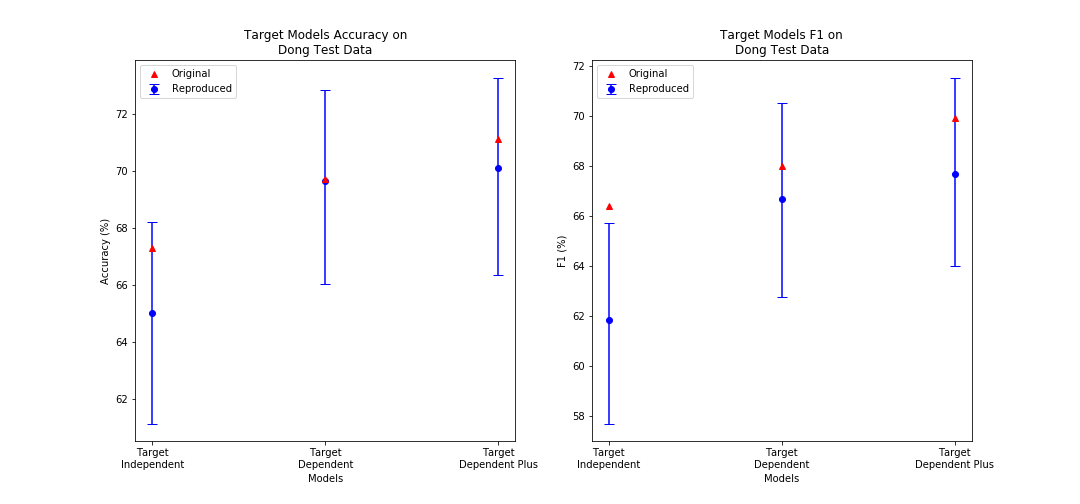
\includegraphics[scale=0.55]{images/reproducibility/Replication_Cases/Target_Replication_Dong.png}
    \caption{Replication of \citet{vo2015target} final experiment.}
    \label{fig:repro_vo_method}
\end{sidewaysfigure}

\subsection{\cite{wang-etal-2017-tdparse}}
%[I actually think he has more than that as they look at the break down of distinct sentiment. Not sure how I am going to get that metric in the theme of the thesis as this was the only paper that actually looked at the TDSA through that metric but it is a very good metric to use I think for TDSA]
The two experiments from this paper are replicated, these test the methods across the test sets of two different Twitter datasets; their own from the politics domain and \citet{dong-etal-2014-adaptive} from the general domain. The C-parameter for the SVM was found in the original paper via grid searching over numerous C-parameters using 5-fold cross validation on the training data, thus the same approach was applied here. The C-parameters were searched using the recommended approach by \citet{hsu2003practical} which is to exponentially grow the C-value, of which there is no recommended starting or ending value, therefore the exponents base used is 2 and the exponent starts at -15 and ends at 2 with a step size of 2 e.g. $C = 2^{-15}, 2^{-13},..., 2^2$, $1$ was also included in the C-parameters as this was the default parameter within the well used scikit-learn library \citep{pedregosa2011scikit}. The best found C-parameter for each method and dataset can be seen in table \ref{table:repro_rep_wang_c}. All other parameters were the same as the original paper except MinMax scaling is also used which was not stated in the original paper but is critical for replication as shown in the parameter settings section \ref{section:repro_effect_param_settings}. As can be seen from figure \ref{fig:repro_wang_dong_method} and \ref{fig:repro_wang_elec_method} all three methods across both datasets and metrics are successfully replicated. The Target Dependent Plus method was not applied to the Election dataset as this experiment was not reported in the original paper.

\begin{table}[]
    \centering
    \begin{tabular}{|c|c|c|c|}
        \hline
         & \multicolumn{3}{|c|}{Methods} \\
        \hline
        Dataset & TDParse Minus & TDParse & TDParse Plus \\
        \hline
        Dong & $2^{-5}$ & $2^{-7}$ & $2^{-7}$ \\
        \hline
        Election & $2^{-7}$ & $2^{-9}$ & $2^{-9}$ \\
        \hline
    \end{tabular}
    \caption{Best C parameters}
    \label{table:repro_rep_wang_c}
\end{table}

\begin{sidewaysfigure}[!ht]
    \centering
    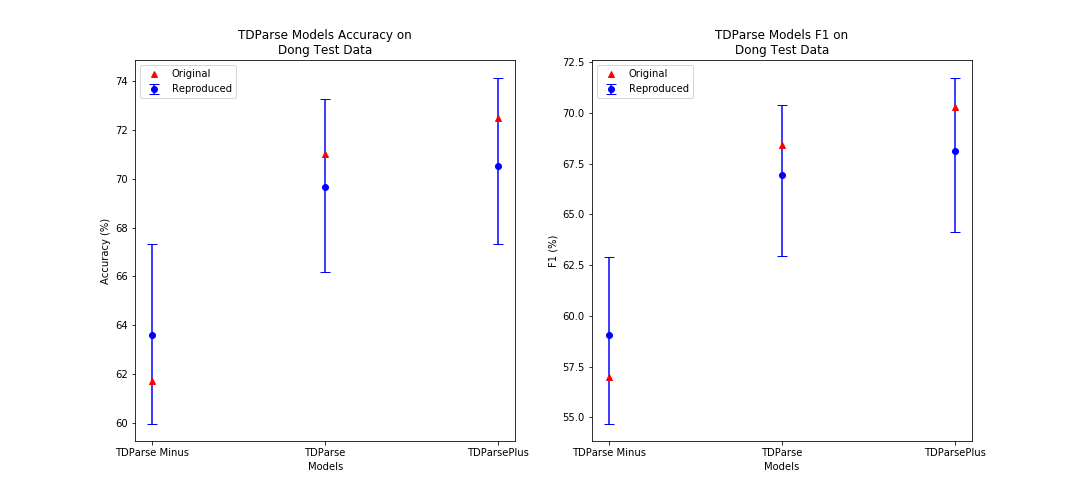
\includegraphics[scale=0.55]{images/reproducibility/Replication_Cases/TDParse_Replication_Dong.png}
    \caption{Replication of \citet{wang-etal-2017-tdparse} on \citet{dong-etal-2014-adaptive} general Twitter dataset.}
    \label{fig:repro_wang_dong_method}
\end{sidewaysfigure}

\begin{sidewaysfigure}[!ht]
    \centering
    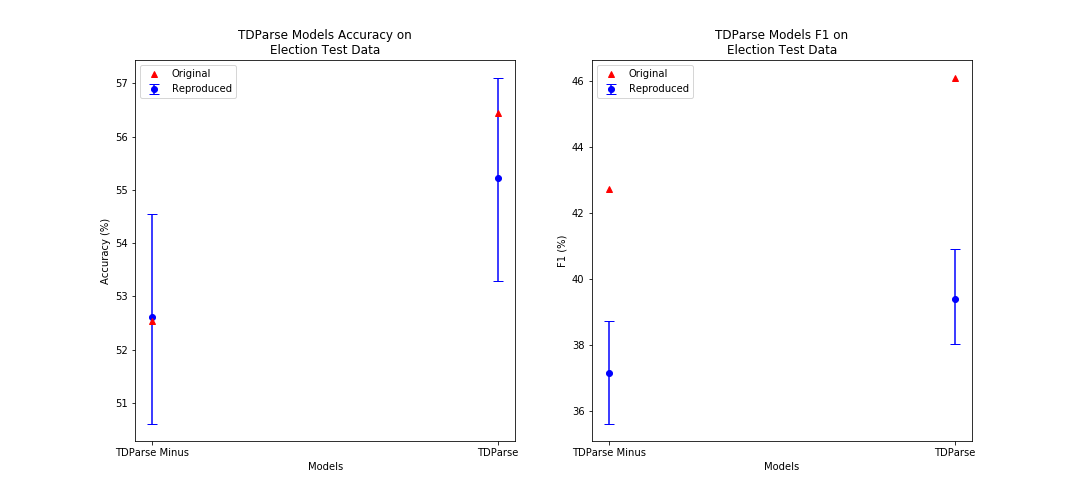
\includegraphics[scale=0.55]{images/reproducibility/Replication_Cases/TDParse_Replication_Election.png}
    \caption{Replication of \citet{wang-etal-2017-tdparse} on \citet{wang-etal-2017-tdparse} political Twitter dataset.}
    \label{fig:repro_wang_elec_method}
\end{sidewaysfigure}

\subsection{Remarks}
To conclude all three methods have been successfully replicated according to hypothesis \ref{hyp:repro_replication_null} and the caveat that only one of the two evaluation metrics had to pass the hypothesis (introduction of section \ref{section:repro_replication}). In the case of replicating \citet{wang-etal-2017-tdparse} on the election dataset using macro F1 metric (figure \ref{fig:repro_wang_elec_method}) the difference between the original and the replicated is quite large. This could be due to the issue of parsing the election dataset, the dataset was constructed in two stages; the first stage the annotators used the targets that were annotated by the three Named Entity Recognition (NER) systems and removed where necessary wrongly annotated targets, the second stage added the targets and sentiment for targets that where annotated by the annotators. This second stage of 688 newly annotated data was not possible to parse of which this would have increased the samples within the positive, neutral, and negative classes by 6.9\%, 3\%, and 7.7\% respectively. Thus this could have caused the differences in the macro F1 score as the relatively large increase for the positive which was the minority class could have made a large difference.



%\subsection{Evaluation}
\section{Effect of Parameter and Experimental \\Settings}
\label{section:repro_effect_param_settings}
All tables within this section that contain survey data, the survey will be of all TDSA papers that; have used the same datasets as those experimented on in this section (listed in table \ref{table:repro_datasets_stats}), and were published after 2013 from one of the following conferences, workshops and journal; 1. ACL, 2. EACL, 3. NAACL, 4. EMNLP, 5. CONLL, 6. COLING, 7. AAAI, 8. TACL, and 9. WASSA. In total their were 31 papers\footnote{The data for this survey can be found here:~\url{https://lancaster.box.com/s/3jsv5qst8cfri6yjklv3tq8lvxzt1o08}}.\\

The following section will look at the affects of changing the following parameters and experimental settings for the methods stated in section \ref{section:repro_methods} while keeping other parameters/settings constant:
\begin{enumerate}
    \item \label{itm:C_SVM} C parameter of the SVM.
    \item \label{itm:Scaling} Scaling the input features before being passed into the SVM.
    \item \label{itm:Senti_lex} Sentiment lexicon(s).
    \item \label{itm:Optimisation} Optimisation algorithm for the NN methods.
    \item \label{itm:TokeniserVectors} Tokeniser and Word Vectors.
\end{enumerate}
The above list contains parameters/settings that are only applicable to certain methods; list items \ref{itm:C_SVM}, \ref{itm:Scaling}, and \ref{itm:Senti_lex} can only be applied to \citet{vo2015target, wang-etal-2017-tdparse}, \ref{itm:Optimisation} can only be applied to \citet{tang-etal-2014-learning}, and \ref{itm:TokeniserVectors} can be applied to all.

This will be the first time within TDSA that the C parameter and sentiment lexicon(s) have been evaluated with significance testing. Previous work \citep{vo2015target} have shown the affects of sentiment lexicons but only through point estimates of which they were marginally different, thus reinforcing the need for significance testing. No work has shown the affect of scaling of which the work that this is evaluated on \citep{vo2015target,wang-etal-2017-tdparse} never stated the need for scaling but it is shown to be critical for replication. There are now numerous optimisation methods for NN, it has been shown within the NER literature \citep{reimers-gurevych-2017-reporting,yang-etal-2018-design} the importance of different optimisation methods thus we use the same setup here to demostarte the importance of these for the first time in TDSA.

In the majority of TDSA papers the tokeniser is never specified, which is shown in table \ref{table:repro_tokeniser_survey}\footnote{If the tokeniser could be found in the paper the code base was not inspected. The unsure category encompasses the cases where; I could not understand the code base confidently, or the task was target extraction and sentiment prediction as the target extraction may have forced the authors to use the pre-tokenised data.}. Therefore compared to the other parameter settings the tokeniser and word vectors are going to be compared jointly to see the affect of using different tokenisers with word vectors that have been created with the same or different tokeniser. Knowing if specifying the tokeniser is important would be a large contribution to the TDSA as so many previous works do not specify the tokeniser.

\begin{table}[h!]
    \centering
    \begin{tabular}{|c|c|}
        \hline
        Category & Count (\%) \\
        \hline
        Paper & 3 (9.7)\\
        \hline 
        Code base & 8 (25.8)\\
        \hline 
        Not at all & 13 (41.9)\\
        \hline 
        Unsure & 7 (22.6)\\
        \hline
        Total & 31\\
        \hline
    \end{tabular}
    \caption{Survey of papers that have either stated the tokeniser in their: paper, code base, not at all, or unsure}
    \label{table:repro_tokeniser_survey}
\end{table}

Word vectors by themselves have also been compared in previous work \citep{vo2015target,tang-etal-2016-effective} without significant tests, and by \citet{marrese-taylor-etal-2017-mining} with significance tests, however the later only evaluated word vectors that have only ever been used in their own and two other works within TDSA\footnote{The word vectors they used were the Senna \citep{collobert2011natural}, GoogleNews \citep{mikolov2013distributed}, and WikiDeps \citep{levy-goldberg-2014-dependency} of which only two previous works have used the GoogleNews vectors \citep{nguyen-shirai-2015-phrasernn,wang-etal-2018-target}} compared to the majority of previous work that has either used Glove \citep{pennington-etal-2014-glove} or SSWE concatenated with TW2V as shown in table \ref{table:repro_survey_word_vector_counts}\footnote{The table counts add to more than 31 (the number of papers) as word vectors are double counted if the paper used them in both review and social media datasets.}. Furthermore as shown by table \ref{table:repro_survey_word_vector_counts} the most common word vector used is Glove 300D, of which this can be either the common crawl 42B or 840B token version. However in the majority of work they do not state which they used simply that they are Glove and 300D, of which this is shown by the survey in table \ref{table:repro_survey_glove_vector_counts}. Therefore in this section these two Glove vectors are compared to see if being vague in which Glove vectors are used is a problem that should be addressed.

\begin{table}[h!]
    \centering
    \begin{tabular}{|c|c|c|}
        \hline
         & Social Media & Review  \\
        \hline 
        Glove 300D & 5 & 16 \\
        \hline 
        SSWE and TW2V & 3 & 0 \\
        \hline 
        Other & 7 & 6 \\
        \hline
    \end{tabular}
    \caption{Survey of dataset types and word vector counts}
    \label{table:repro_survey_word_vector_counts}
\end{table}

\begin{table}[h!]
    \centering
    \begin{tabular}{|c|c|c|}
        \hline
        Vector & Count (\%)  \\
        \hline 
        Glove 42B & 3 (17.6)\\
        \hline 
        Glove 840B & 4 (23.5)\\
        \hline 
        Glove 300D & 10 (58.8)\\
        \hline
    \end{tabular}
    \caption{Survey of 300D Glove vectors and how they are stated in papers}
    \label{table:repro_survey_glove_vector_counts}
\end{table}

Domain specific word vectors have been applied all within the Twitter based datasets \citep{mitchell-etal-2013-open,dong-etal-2014-adaptive,wang-etal-2017-tdparse} using SSWE or/and TW2V \citep{vo2015target,tang-etal-2016-effective,zhang2016gated,wang-etal-2017-tdparse}, or Glove vectors trained on Twitter (GloveTwit) \citep{tang-etal-2016-effective}, or custom word vectors \citep{zhang-etal-2015-neural}. Thus in this section domain specific word vectors will be evaluated accross numerous datasets that go outside of the Twitter domain. This would be a first within TDSA to see the affect of domain specific compared to general word vectors.\\


In this section we are going to follow the list above thus the first subsection is showing the affect the C parameter has and the last is on tokenisers and word vectors. In all subsections all other parameters apart from the one being tested will be fixed, in the ideal case no parameters would be fixed and all permutations would be tested, however this would be computationally infeasible. All the parameters will be tested across multiple datasets which are shown in tables \ref{table:repro_datasets_stats} and \ref{table:repro_dataset_sent_dist}, thus they will be tested across many and varying dataset properties. The following parameters and their values will be fixed as specified until they are evaluated:
\begin{enumerate}
    \item Tokeniser -- Stanford. 
    \item Word Vectors -- Glove common crawl 840B (Glove 840B).
    \item Scaling -- MinMax.
    \item Dependency parser -- TweeboParser.
    \item Sentiment Lexicons -- The union of MPQA, HL, and NRC which were processed in the same way as \citet{vo2015target}\footnote{This processing was: the union of the lexicons filtering all words that contain opposing sentiments.}.
\end{enumerate}
This tokeniser was chosen as it was the tokeniser used in the creation of the Glove 840B vectors. The Glove 840B vectors are the most popular vectors with the 42B version, but compared to the 42B version they were trained on a larger corpus thus more likely to have better word representation and they have a larger vocabulary. MinMax scaling compared to no scaling has been shown to be benifical \citep{moore-rayson-2018-bringing}. The dependency parser is the one used in the original paper. Lastly as all sentiment lexicons were used in \citet{wang-etal-2017-tdparse} and found to be marginally worse than the best combination in \citet{vo2015target}. Once a parameter has been evaluated the best found parameter for each method and dataset will be used for the subsequent evaluations. For all parameter evaluations the test data will never be used to ensure no overfitting to the test data. 

\afterpage{%
    \clearpage% Flush earlier floats (otherwise order might not be correct)
    \thispagestyle{report}
    \begin{landscape}% Landscape page
        \centering % Center table
        \begin{tabular}{|c|c|c|c|c|c|c|c|c|c|c|}
            \hline
            Dataset & Domain & Type & Size & Medium & ATS & Uniq & AVG Len & S1 & S2 & S3\\
            \hline
            \hline
            SemEval 14 L& L & RE & 2951 & W & 1.58 & 1295 & 18.57 & 81.09 & 17.62 & 1.29 \\
            \hline
            SemEval 14 R& R & RE & 4722 & W & 1.83 & 1630 & 17.25 & 75.26 & 22.94 & 1.80 \\
            \hline
            Mitchel & G & S & 3288 & W & 1.22 & 2507 & 18.02 & 90.48 & 9.43 & 0.09 \\
            \hline
            Dong Twitter& G & S & 6940 & W & 1.00 & 145 & 17.37 & 100.00 & 0.00 & 0.00 \\
            \hline
            Election Twitter& P & S & 11899 & W & 2.94 & 2190 & 21.68 & 44.50 & 46.72 & 8.78 \\
            \hline
            YouTuBean& MP & RE/S& 798 & SP & 2.07 & 522 & 22.53 & 81.45 & 18.17 & 0.38 \\
            \hline
            \hline
            \multicolumn{11}{|p{\linewidth}|}{L=Laptop, R=Restaurant, G=General, P=Politics, MP=Mobile Phones, RE=Review, S=Social Media, W=Written, SP=Spoken, ATS=Average Targets per Sentence, Uniq=No. unique targets, AVG len=Average sentence length per target, S1=1 distinct sentiment per sentence, S2=2 distinct sentiments per sentence, S3=3 distinct sentiments per sentence}\\
            \hline
        \end{tabular}
        \captionof{table}{Dataset Statistics}
        \label{table:repro_datasets_stats}
    \end{landscape}
    \clearpage% Flush page
}
 






\subsection{SVM C Parameter}
\label{section:repro_param_c_value}

This is the first parameter of the linear SVM methods that will be evaluated therefore the evaluation setup of the linear SVM parameters only will be explained first. The second part of this subsection will introduce what the C parameter is, the C paramters that are going to be evaluated, as well as the results.\\

As it is typical for SVM based methods to tune their parameters with cross validation, of which five fold cross validation was used in \citet{vo2015target} and \citet{wang-etal-2017-tdparse} for parameter tuning this is what will be used here. As the results will be reported for each method trained and tested over five folds of each dataset, the significance testing setup that was introduced in subsection \ref{section:repro_replication} needs revising. The revision is required as in the previous setup the testing was only on one dataset where as here the five folds, effectively creates five datasets thus this would create five p-values for each method on each dataset. Therefore in this evaluation setup instead of stating if the results are significant for a method on a dataset, the number of folds that are significant will be reported for each method and dataset. However using the simple approach of counting the number of folds that are less than some $\alpha$ has been shown to introduce more type 1 errors \citep{dror-etal-2017-replicability} than that was set by the $\alpha$ parameter in the individual significance tests. Therefore to stop the introduction of type 1 errors and keep the upper bound to $\alpha$ a correction procedure is required of which \citet{dror-etal-2018-hitchhikers} recommends two; Fisher and Bonferroni \citep{benjamini2008screening}. The difference between the two is that Fisher should be used when the p-values have come from datasets that are independent, where as Bonferroni can be used for dependent datasets. As each fold does depend on the other folds the Bonferroni correction will be used here. The p-value for each fold will still be calculated using the paired bootstrap test that was introduced in subsection \ref{section:repro_replication}. What was generally introduced here was significance testing for multiple datasets.\\

The C-parameter is part of the L2-regularised L2-loss function of the linear SVM which can be seen in equation \ref{eq:repro_svm} (taken from equation 2 in \citep{fan2008liblinear}). The L2-regulisation in the equation is $\frac{1}{2}w^Tw$ and the rest is the L2-loss. As can be seen the C parameter determines the amount of weight the L2-loss has on the overall loss function. Thus if the C parameter is large the effect of the regulisation is small, which would more likely cause the model to overfit to the training data making it less generalisable.
\begin{equation}
    \frac{1}{2}w^{T}w + C\sum_{i=1}^{l}(\max(0, 1 - y_{i}w^{T}x_i))^2
    \label{eq:repro_svm}
\end{equation}
The C-parameters that are going to be tested for per method across all datasets are the same as those evaluated for the replication of \citet{wang-etal-2017-tdparse} in subsection \ref{section:repro_replication}. 

The results for the accuracy and macro F1 metric can be seen in figures \ref{fig:repro_param_c_sig_acc} and \ref{fig:repro_param_c_sig_f1}. Before analysing the results from these figures, the figures will be explained. Each method is trained and tested five times, once for each fold, for every C parameter as stated earlier. For each method and dataset the best performing C-parameter is found through averaging the metric values across all five folds, this best C-parameter is represented by the coloured dots in the figures. As the paired bootstrap test can only compare one method to another, the mean best C-parameter is compared to all other C-parameters where the null hypothesis is;
\textit{The mean best C-parameter is no better than the other C-parameter}. Compared to the paired bootstrap test of section \ref{section:repro_replication} this would be a one tailed t-test rather than two. The cross within the figures are therefore the number of times the mean best C-parameter is significantly better than the other C-parameter, where the five significant values from performing the significant test on each fold is corrected using Bonferroni.

Interestingly when comparing the results across the two metrics the results differ a lot, more so for datasets that are more un-balanced dataset e.g. Mitchell and YouTuBean compared to those that have a more balanced dataset e.g. Dong and SemEval 14 L. This is expected to some extent as the macro F1 score treats each the F1 score for each class equally and the expectation is that the SVM wants to find the maximum separation between the classes. Where as for accuracy it is best in the un-balanced dataset to find the C parameter that separate between the majority class and the other classes therefore a more general separation is best. This difference between the F1 and accuracy can also be seen more explicitly in the average performance plots in figures \ref{fig:repro_param_avg_f1} and \ref{fig:repro_param_avg_acc} where the F1 scores for all methods and datasets perform a lot worse at the lower C parameters compared to the larger C parameters. As one of the C parameters $1$ is the default value in scikit-learn it is interesting that the default value is often statistically significantly worse than the best C parameter across both metrics\todo{look here} (6) demonstrating the need to tune the C parameter to the relevant task as expressed by numerous authors \citep{fan2008liblinear,vo2015target,wang-etal-2017-tdparse}. Compared to \citet{vo2015target} who also tuned the C parameter and reported their results but without significance testing using five fold cross validation, the findings here are comparable.
\begin{sidewaysfigure}[!htb]
    \centering
    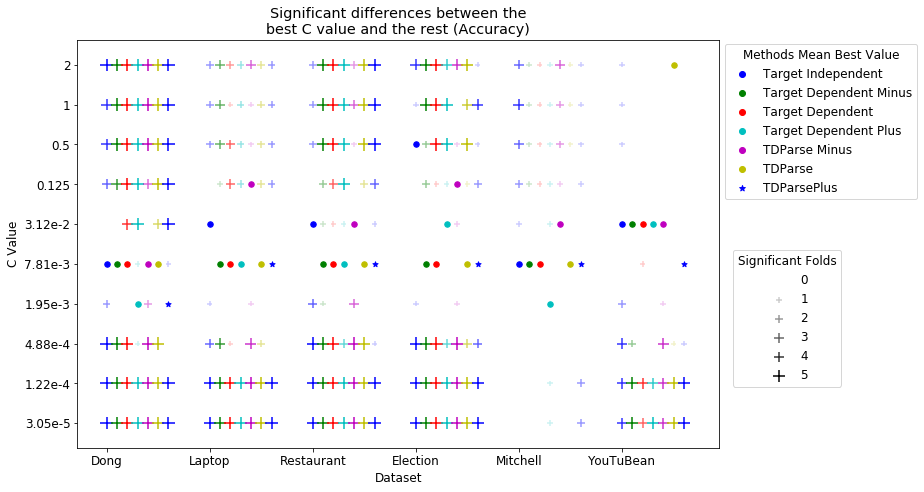
\includegraphics[scale=0.55]{images/reproducibility/Parameters/C_Parameter/C_Sig_Plot_Accuracy.png}
    \caption{C parameters significance results (accuracy)}
    \label{fig:repro_param_c_sig_acc}
\end{sidewaysfigure}
\begin{sidewaysfigure}[!htb]
    \centering
    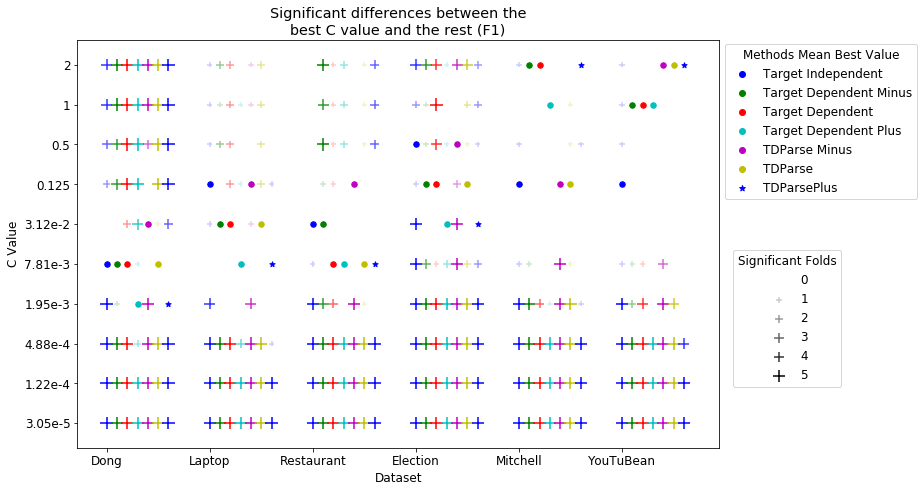
\includegraphics[scale=0.55]{images/reproducibility/Parameters/C_Parameter/C_Sig_Plot_F1.png}
    \caption{C parameters significance results (macro F1)}
    \label{fig:repro_param_c_sig_f1}
\end{sidewaysfigure}
\begin{figure}[!htb]
    \centering
    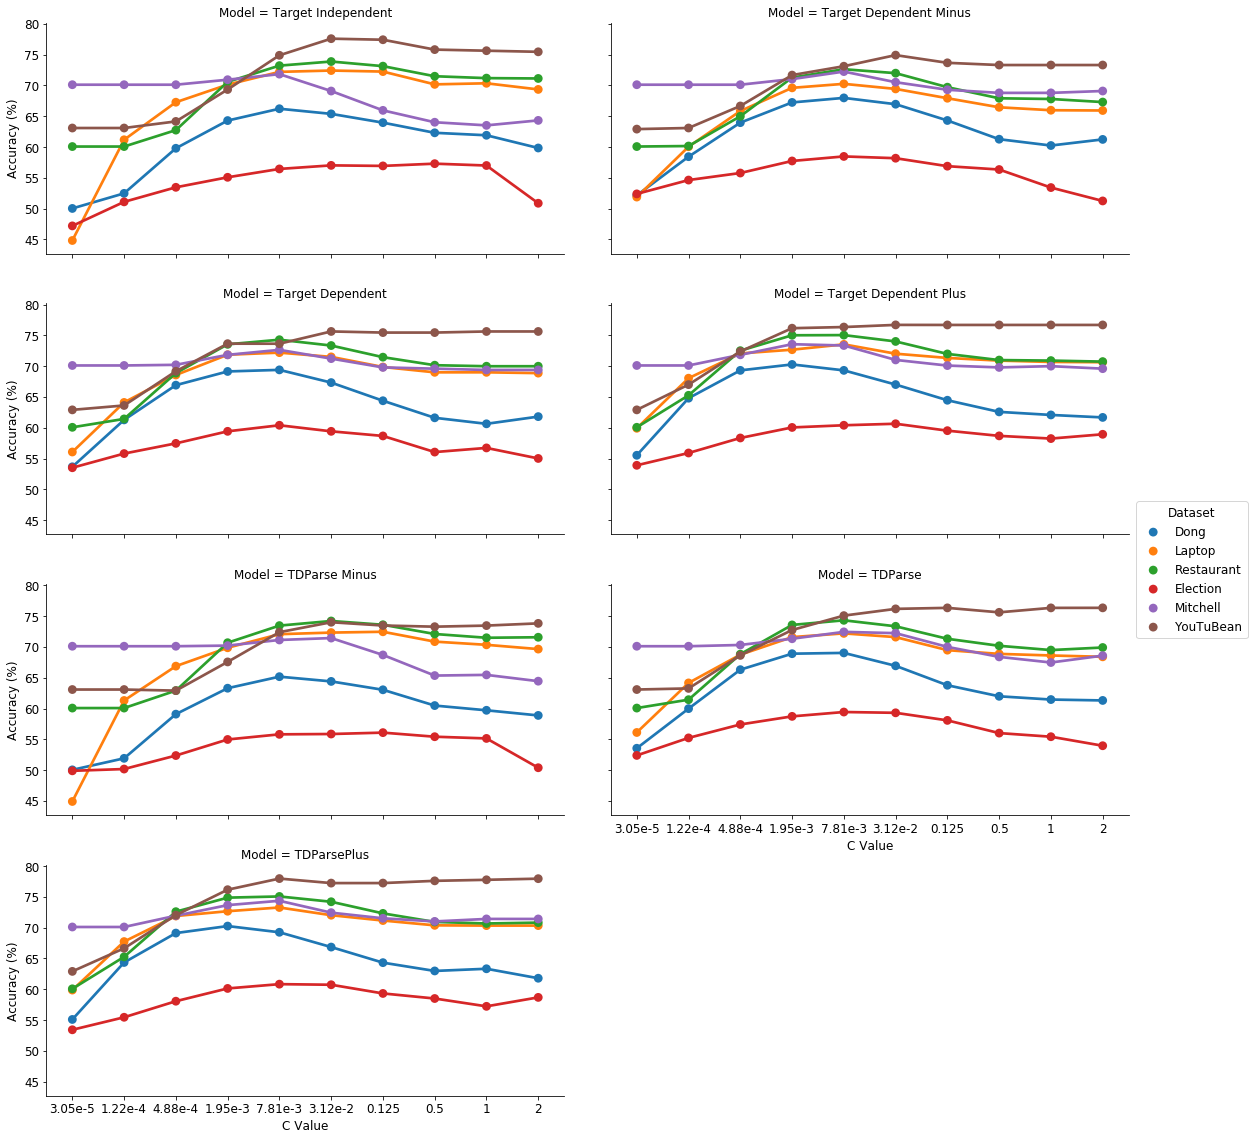
\includegraphics[scale=0.3]{images/reproducibility/Parameters/C_Parameter/C_Accuracy_Plot.png}
    \caption{C parameters average accuracy score across five folds}
    \label{fig:repro_param_c_avg_acc}
\end{figure}
\begin{figure}[!htb]
    \centering
    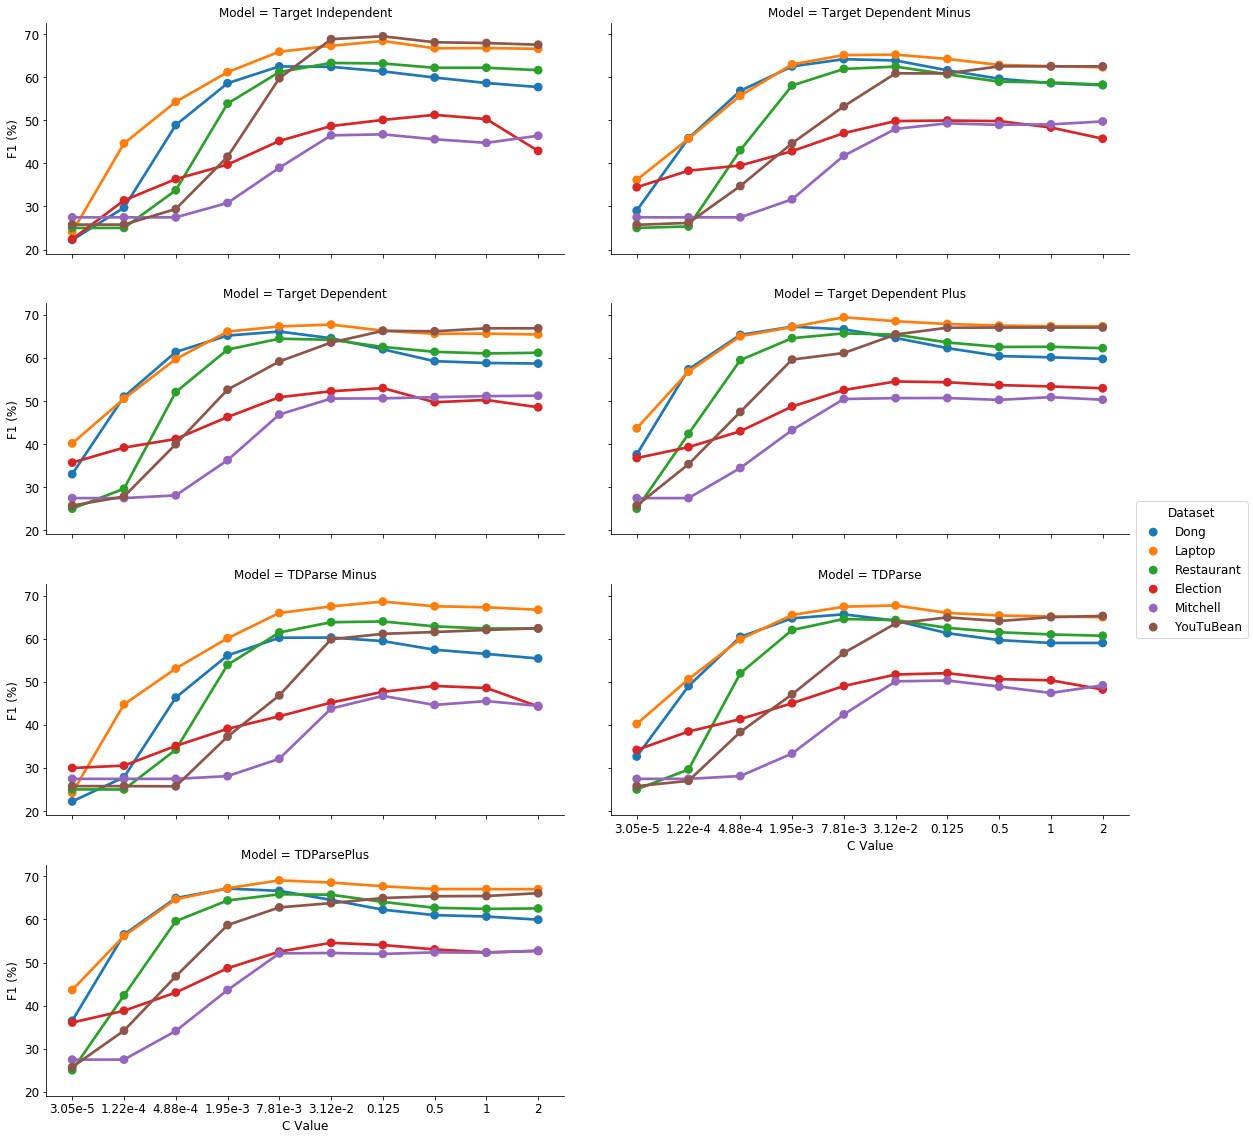
\includegraphics[scale=0.3]{images/reproducibility/Parameters/C_Parameter/C_F1_Plot.png}
    \caption{C parameters average macro F1 score across five folds}
    \label{fig:repro_param_avg_f1}
\end{figure}

\newpage
\FloatBarrier
\subsection{Scaling}
Using the same evaluation setup as that in the previous section \ref{section:repro_param_c_value}, the scaling of the features before being inputted into the SVM is being experimented here. Only two types of scaling are going to be experimented here the MinMax scaling and no scaling at all. MinMax scaling scales each features into a pre-defined \textit{max} to \textit{min} range, this therefore reduces the affects of outliers within the feature range and allows the values between the features to be more comparable. MinMax scaling as shown in equation \ref{eq:repro_min_max_scaling} where $X$ is a feature vector for all samples, $X_{min}$ and $X_{max}$ are the smallest largest value respectively in the feature vector can scale the data between any \textit{max} and \textit{min} range of which in the experiments shown throughout this thesis \textit{max} is $1$ and \textit{min} is $0$.
\begin{equation}
    X = \frac{X - X_{min}}{X_{max} - X_{min}} * (max - min) + min
    \label{eq:repro_min_max_scaling}
\end{equation}

The results showing which scaling method is significantly better than the other for accuracy and macro F1 can be seen in figures \ref{fig:repro_param_scale_sig_acc} and \ref{fig:repro_param_scale_sig_f1} respectively. As can be seen by both metrics across all methods and all but the Mitchell dataset scaling your features is statistically significantly better than not scaling.
\begin{figure}[!htb]
    \centering
    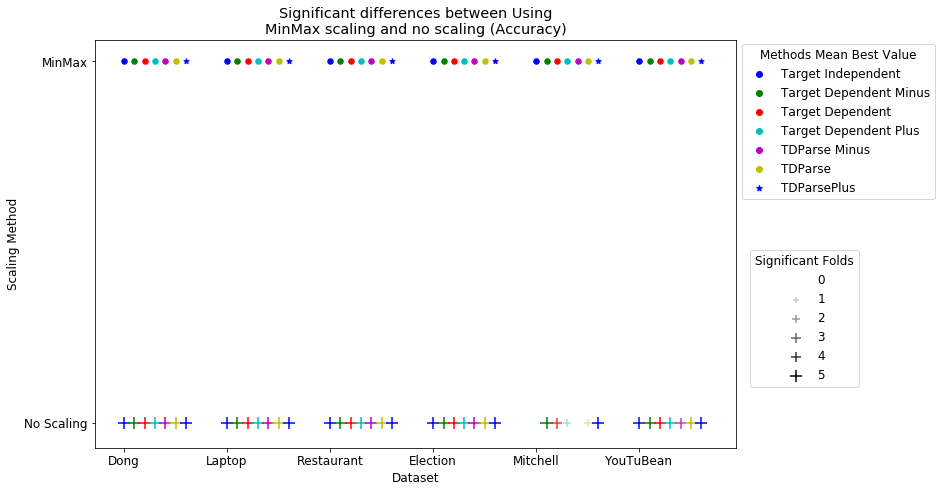
\includegraphics[scale=0.4]{images/reproducibility/Parameters/Scaling/Scaling_Sig_Plot_Accuracy.png}
    \caption{Scaling parameter accuracy}
    \label{fig:repro_param_scale_sig_acc}
\end{figure}
\begin{figure}[!htb]
    \centering
    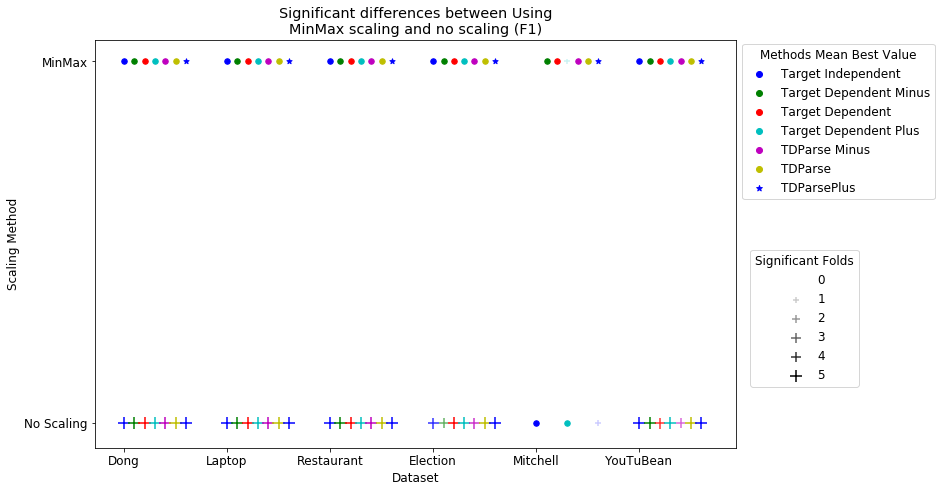
\includegraphics[scale=0.4]{images/reproducibility/Parameters/Scaling/Scaling_Sig_Plot_F1.png}
    \caption{Scaling parameter F1}
    \label{fig:repro_param_scale_sig_f1}
\end{figure}
Furthermore the replication experiments for \citet{vo2015target} and \citet{wang-etal-2017-tdparse} have been re-created but without scaling the features, this can be seen in figures and shows that without scaling in the majority the of the results would not reproduce the original findings.
\begin{figure}[!htb]
    \centering
    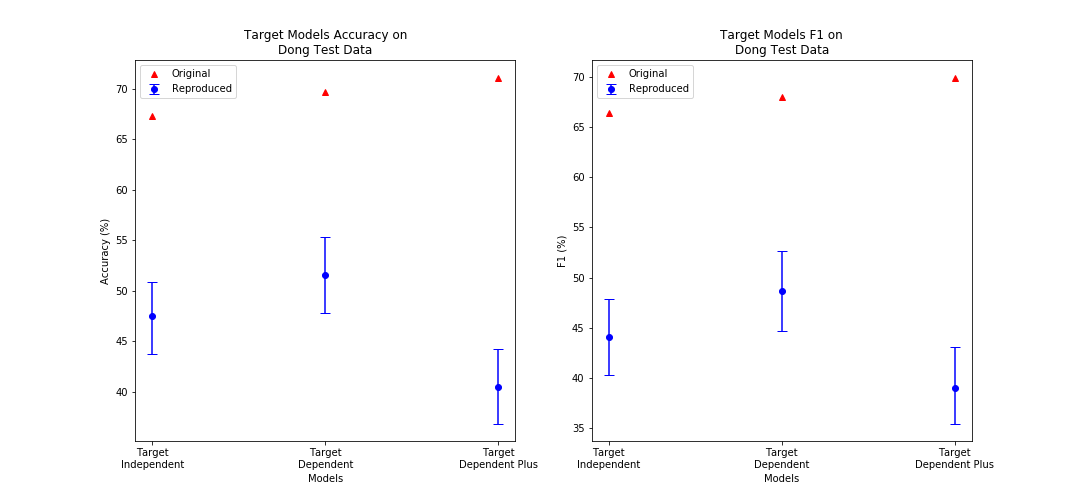
\includegraphics[scale=0.35]{images/reproducibility/Parameters/Scaling/Target_Replication_not_scaled_Dong.png}
    \caption{\citet{vo2015target} experiment replicated without scaling the features}
    \label{fig:repro_param_scaling_target_exp}
\end{figure}
\begin{figure}[!htb]
    \centering
    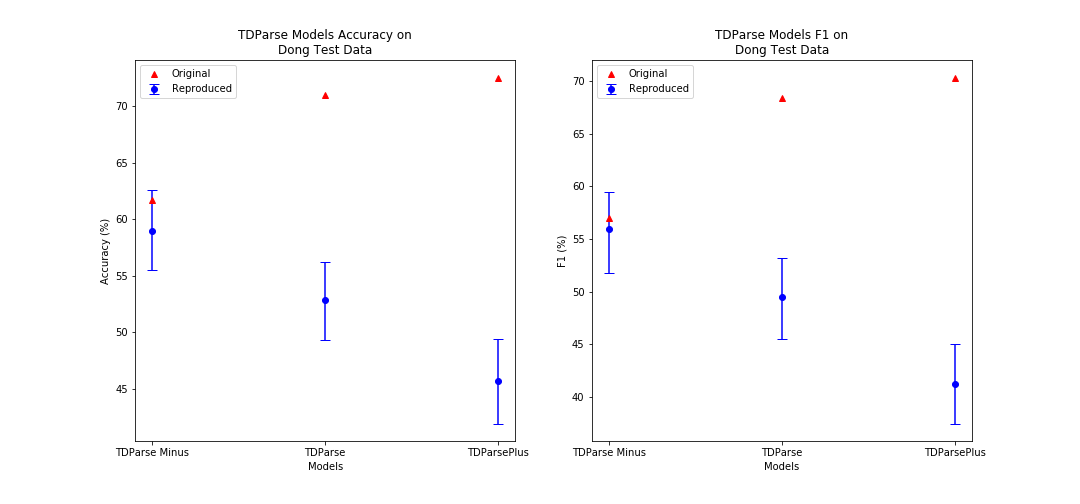
\includegraphics[scale=0.35]{images/reproducibility/Parameters/Scaling/TDParse_Replication_not_scaled_Dong.png}
    \caption{\citet{wang-etal-2017-tdparse} experiment replicated on the Dong Twitter dataset without scaling the features}
    \label{fig:repro_param_scaling_tdparse_dong}
\end{figure}
\begin{figure}[!htb]
    \centering
    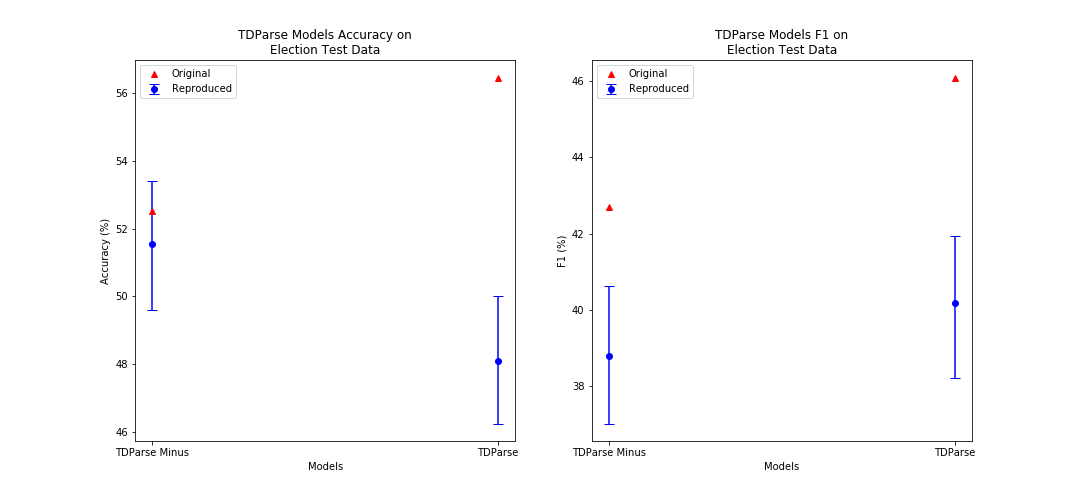
\includegraphics[scale=0.35]{images/reproducibility/Parameters/Scaling/TDParse_Replication_not_scaled_Election.png}
    \caption{\citet{wang-etal-2017-tdparse} experiment replicated on the Election Twitter dataset without scaling the features}
    \label{fig:repro_param_scaling_tdparse_election}
\end{figure}
As stated earlier in this section \ref{section:repro_effect_param_settings} none of the previous work that use SVM's that have been replicated here clearly define in their paper that scaling is being used. \citet{wang-etal-2017-tdparse} code base does show that they use scaling. Also both \citet{vo2015target} and \citet{wang-etal-2017-tdparse} state that they use the LibLinear library \citep{fan2008liblinear} of which they do recommend both in their practical guide \citep{hsu2003practical} and paper \citep{fan2008liblinear} to scale the data before using the SVM. However neither of the papers state scaling in the paper and considering how important this setting is to replicate their experiments it would be recommended to state in the paper in the future and not just the code base or as assumption based on a SVM library recommendations.
\newpage
\FloatBarrier
\subsection{Sentiment Lexicons}
Two of the methods in \citet{vo2015target} and \citet{wang-etal-2017-tdparse} use sentiment lexicons, of which these methods are \textit{Target Dependent Plus} and \textit{TDParse Plus} respectively. The sentiment lexicons used were the union of the MPQA, HL, and NRC for \citet{wang-etal-2017-tdparse}, where as \citet{vo2015target} used the union of MPQA and HL as they found this to be best. However \citet{vo2015target} only compared the different combination of sentiment lexicons with point estimates and did not state if this best combination was significantly better than the rest.

The results showing whether the best found sentiment lexicon is significantly better than the rest for both accuracy and macro F1 can be seen in figures \ref{fig:repro_param_senti_lex_sig_acc} and \ref{fig:repro_param_senti_lex_sig_f1} respectively. As can be seen the best sentiment lexicon in the majority of the cases is not significantly better than any other sentiment lexicon. 
\begin{figure}[!htb]
    \centering
    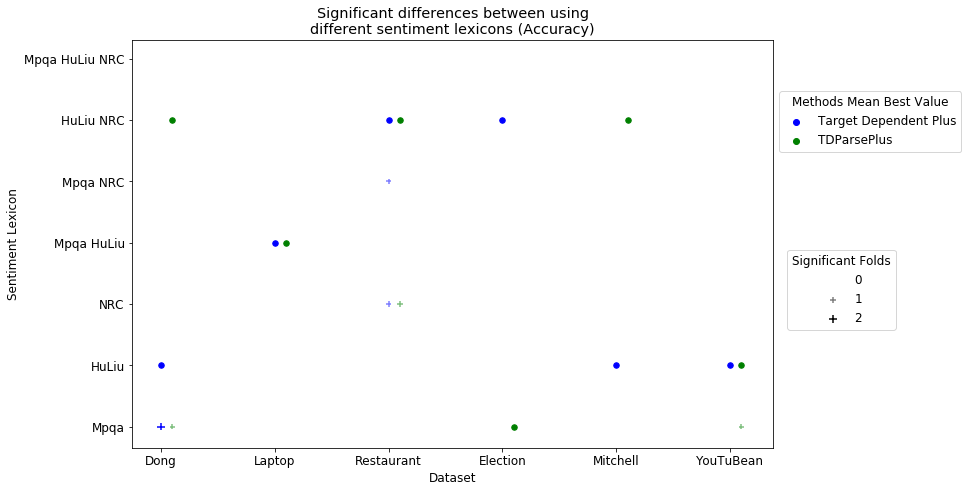
\includegraphics[scale=0.4]{images/reproducibility/Parameters/Sentiment_Lexicons/Sentiment_Lexicon_Sig_Plot_Accuracy.png}
    \caption{Sentiment lexicon parameter accuracy}
    \label{fig:repro_param_senti_lex_sig_acc}
\end{figure}
\begin{figure}[!htb]
    \centering
    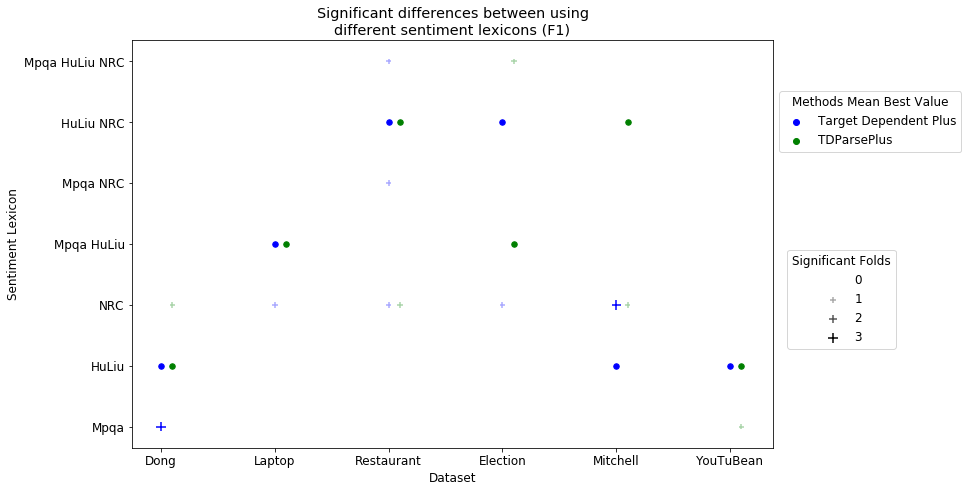
\includegraphics[scale=0.4]{images/reproducibility/Parameters/Sentiment_Lexicons/Sentiment_Lexicon_Sig_Plot_F1.png}
    \caption{Sentiment lexicon parameter F1}
    \label{fig:repro_param_senti_lex_sig_f1}
\end{figure}
This shows that even though normally sentiment lexicons help improve performance as shown in figures \ref{fig:repro_param_senti_lex_avg_acc} and \ref{fig:repro_param_senti_lex_avg_f1}, this improvement is not significant.
\begin{figure}[!htb]
    \centering
    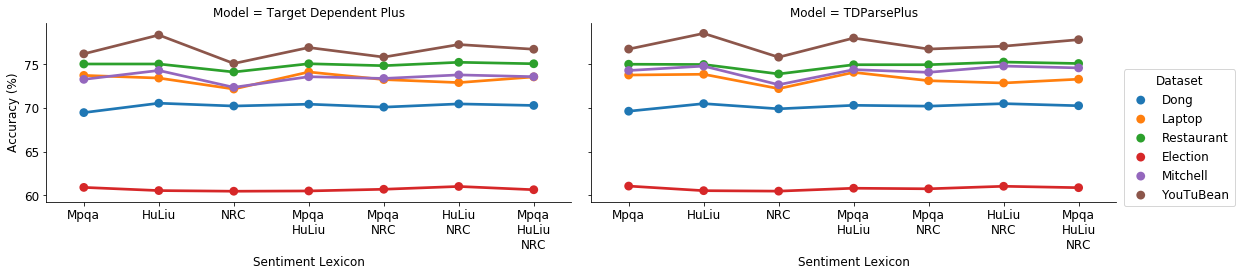
\includegraphics[scale=0.3]{images/reproducibility/Parameters/Sentiment_Lexicons/Sentiment_Lexicon_Accuracy_Plot.png}
    \caption{Sentiment lexicon average accuracy score across five folds}
    \label{fig:repro_param_senti_lex_avg_acc}
\end{figure}
\begin{figure}[!htb]
    \centering
    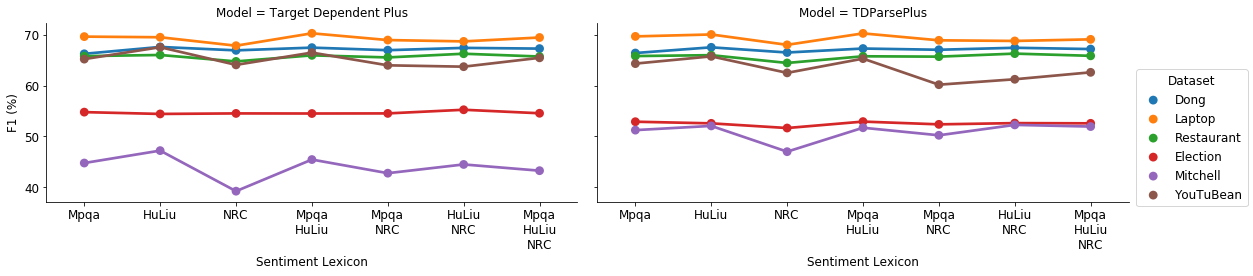
\includegraphics[scale=0.3]{images/reproducibility/Parameters/Sentiment_Lexicons/Sentiment_Lexicon_F1_Plot.png}
    \caption{Sentiment lexicon average accuracy score across five folds}
    \label{fig:repro_param_senti_lex_avg_f1}
\end{figure}
\newpage
\FloatBarrier
\subsection{Neural Network Optimiser}
\subsection{Validation Set?}
\subsection{Tokenisation and Word Vectors}
\section{Mass Evaluation}
\section{Conclusion}
Mention the link between the parameter settings evaluation and replication sections through scaling, if the scaling parameter was never adjusted it would not have been possible to successfully replicate the methods.
\label{section:repro_mass_eval}

\section{Some other research}
Papers of interest on reproducibility within the machine learning community that can be found in this good blog post that is relevant \url{https://ai.facebook.com/blog/how-the-ai-community-can-get-serious-about-reproducibility/}